\chapter{Evaluation}
\label{chapter:evaluation}

\section{Methodology}

\subsection{Goals}

Recall our research questions.

\begin{enumerate}
    \item By how much can the cold-start problem be alleviated under the Wasm runtimes?
  
    \item How do the performance characteristics of the Wasm and container runtimes differ?
  
    \item What are the resource costs for keeping functions warm in both approaches?
  
    \item Which Webassembly runtime is most suitable for the use on heterogeneous edge devices?
\end{enumerate}

These questions guide our evaluation approach. First we describe the type of workload we run on OpenWhisk in both its base version and its modified Wasm version. Then we describe how our measurements are taken and how we evaluate each of the research questions. 

\subsection{Workload Types}

To measure the performance of the serverless platform in a meaningful way, we reviewed the literature for use cases, where latency is critical; in turn, where the cold start time matters most. From these examples as well as characterizations of the workload types in section \ref{section:serverless_workload}, we infer an evaluation workload.

\begin{description}[style=multiline, leftmargin=2.5cm, font=\bfseries]

    \item[Vital Signs Analysis] \citeauthor{Nastic2017} introduce measuring a patient's vital signs as a latency-critical application. Decisions must be made quickly so it serves as an example, where a serverless platform on edge computers can provide lower latency than sending the data to the cloud \cite{Nastic2017}. Thus, part of the latency is reduced by physically moving the serverless platform closer to the edge device. However, the second important factor for latency is the platform's execution latency, i.e. its cold start time. Reducing the latter from multiple seconds down to a few milliseconds can make an important difference in that use case. The workload is data analytics, which can be classified as CPU-bound, because of the involved data preprocessing, analysis and perhaps even machine learning model training.
    \item[Edge AI] \citeauthor{Rausch2019} describe a motivational use cases for AI at the serverless edge. The first is similar to the just-introduced example. A personal bio sensor measures blood sugar levels and sends it to an edge device, which refines a pre-trained model with that data and serves the model for inferencing \cite{Rausch2019}. The workload for this type of serverless function needs a significant amount of CPU-time for the machine learning tasks but also writes and reads parts of the model to and from disk. This workload cannot be unambiguously classified as either CPU- or file-I/O-bound, as it is rather both at once.
    \item[APIs] According to \citeauthor{Eismann2021a} -- who conducted a manual analysis of serverless applications -- 28\% of their analysed applications were APIs \cite{Eismann2021a}. Even with today's cold start latency, developers are already using serverless for user-facing applications, where latency is rather important. If the latency could be reduced, even latency-critical APIs may be able to use serverless. A useful API is typically accessing or modifying state. Since serverless functions are stateless, they need to communicate with other services such as databases, event buses, logging services or they might even call other functions. This composition can be classified as network-I/O-bound, since the function spends most of its time waiting for the call to the external resource to complete.

\end{description}

We infer two workloads from these. Both CPU- and network-I/O-bound workloads are a primary type that ought to be handled well by a serverless platform. Some limitations apply due to WASI's immaturity or serverless idiosyncracies. In particular, to model a full machine learning example, we should access an already trained model and run predictions on it. However, due to the lack proper network accessibility in WASI we cannot retrieve it from an external service. Due to vanilla OpenWhisk using Docker containers, storing the model on disk would require granting each container access to the model's path on the host, which is not trivially done. We write the actions in Rust and compile it to the \inl{wasm32-wasi} and \inl{aarch64-unknown-linux-musl} target respectively, depending on whether we run a WebAssembly-based executor or the Docker-based one. This ensures that our results aren't distorted by two different implementations in separate languages. It is also one less parameter to take into account when reasoning about the results. In order to execute the native binary in OpenWhisk, we use its blackbox feature. It is implemented by its \inl{dockerskeleton} image, which lets us execute any action that adheres to a JSON-in, JSON-out protocol. We could also use the official Rust support by OpenWhisk, however, that takes a Rust source file and compiles it during the initialization phase, massively distorting the cold start latency. We think using the blackbox version makes for a fair comparison between both container runtime types.
OpenWhisk makes its docker runtime images available for the \inl{x86\_64} architecture only, so we need to build this image for \inl{aarch64}\footnote{\url{https://hub.docker.com/r/pgackst/dockerskeleton}}, in order to execute on our Raspberry Pi. The concrete implementations of our evaluation actions are the following programs.

\begin{description}[style=multiline, leftmargin=2.5cm, font=\bfseries]
    \item[CPU-bound] For this workload, we repeatedly hash a bytestring in a loop using the \inl{blake3} \todo{blake3 footnote} algorithm. This is a convenient choice since its reference implementation is in Rust. Hashing is CPU-bound and free from system calls, so it is a good candiadate for this workload type. We choose the number of iterations so that the completion takes roughly 100ms on the native system, in order to have a non-trivial amount of work to be done for each invocation -- more than OpenWhisk needs for its scheduling internally.
    \item[Network-I/O-bound] For this workload we make an HTTP request to a local server which always takes exactly 100ms to complete.
\end{description}

% Note that we deliberately do not use no_std or other mechanisms to make the modules small, so as to represent a real-world applicable use-case where Rust's std library would most likely be used

\subsection{Setup}

We want to measure the cold start latency and action execution time across all our evaluations. To that end, we utilize OpenWhisk's activation record, which is a collection of data resulting from each action invocation.  Recall that OpenWhisk either initializes and runs the action, in the case of a cold start, or skips the initilization and runs it in a warm container. Each activation record contains a \inl{waitTime} annotation, which is the time between the arrival of the request and the provisioning of a container. It's important to note, that this applies only to docker, since a Wasm container is only represented as a Wasm module, which is created during the initialization. However, the \inl{waitTime} does not include that initialization time, which is recorded as a separate annotation: \inl{initTime}. Thus, for a fair comparison between both container runtimes, we define the cold start time as \inl{waitTime + initTime}. Measured this way, the cold start time is simply the time between OpenWhisk receiving the request and the container being ready for execution. Since both times are part of the latency the user perceives, we believe this to be an accurate measurement. It's important to note that this allows for a fair comparison in relative terms, but the recorded cold start times are not made up entirely of the container runtimes' startup cost, but also of OpenWhisk internals, which may account for a significant portion.

The record also contains a \inl{duration} field which is the duration of the entire execution, including the potential \inl{initTime}. To measure the pure performance of the container runtimes, we subtract \inl{initTime} from \inl{duration}, if necessary. In figure \ref{fig:evaluation-time-measurement} we show an overview of measurements we calculate.

\begin{figure}
    \begin{center}
        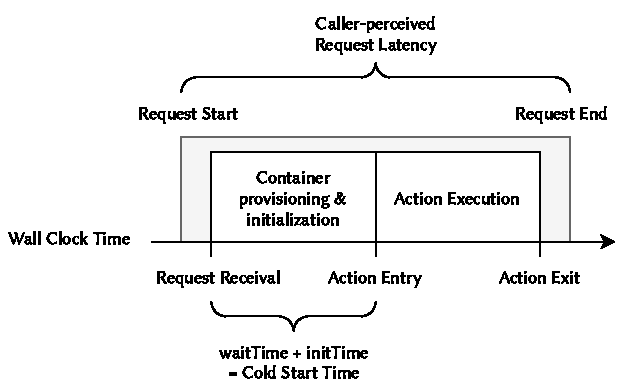
\includegraphics{figures/EvaluationTimeMeasurement.pdf}
    \end{center}
    \caption{The two durations we calculate to measure the system's performance.}
    \label{fig:evaluation-time-measurement}
\end{figure}

% With this setup alone, it is difficult to measure the cold start latency, since end - start would include the execution time. To lift this restriction, we additionally measure the wall clock time inside the action, when it enters its main function. Furthermore -- to maximize precision -- we also measure the timestamp at which the main function exits and ignore the activation end timestamp as a result. That leads us to our setup in figure \ref{fig:evaluation-time-measurement}. Now we can accurately measure the time it takes to get the underlying container technology initialized by taking the difference of the entry and start timestamp.

% start - end includes Wasm module's memory allocation and serialization, could mention that and reference its description in the design chapter
% Possibly cite https://www.sciencedirect.com/science/article/pii/B9780124201583000137?via%3Dihub



There are a few papers measuring serverless performance which also describe their approach in more detail. We use those as a basis for our evaluation.

\begin{itemize}
    \item \citeauthor{McGrath2017} use concurrency and backoff tests. The concurrency test starts by issuing a request to the platform and reissues it as soon as it completes. At a fixed interval, it adds another request up to an upper bound. The performance metric is responses per second. The backoff test measures cold start times by issuing single requests at increasing intervals, in order to trigger the platforms deallocation of warm containers \cite{McGrath2017}.
    \item \citeauthor{Hall2019} characterize serverless function access patterns based on a real-world scenario. They describe three different patterns: Non-concurrent requests from a single client; multiple clients making a single request, possibly concurrent; multiple clients making multiple requests, possibly concurrent \cite{Hall2019}.
\end{itemize}

In the interest of reducing complexity, we will run multiple evaluations and measure for the least amount of dimensions. Those evaluations are:

\begin{itemize}
    \item For the cold start latency evaluation we will send concurrent requests to our deployment. The goal is to examine the effect of the Wasm runtime's execution model (i.e. JIT, AoT or interpreted) on the cold start latency.
    We also run it against the Docker-based baseline OpenWhisk. We use a similar approach as \citeauthor{McGrath2017} in their backoff test. That is, in each step, sending $i$ concurrent requests and waiting for complete container deallocation inbetween steps, in order to trigger $i$ cold starts in every test. We run $N$ tests, so that $i \in {1..N}$ and $N$ is the upper bound we determine during the tests. We only use the CPU-bound workload, because the workload type does not matter for the cold start. 
    In our case, we can fix the interval, since we can configure the deallocation time as well. Specifically, we set the \inl{idle-container} timeout to 10 seconds, meaning that OpenWhisk will remove the container after 10 seconds if no suitable request has come in during that time. This measurement will aid in answering research question 1.

    \item To evaluate the performance of the system we will run concurrent requests against an edge device under a mixed workload consisting of equal amounts of CPU- and I/O-bound actions. We repeat this measurement for all our Wasm runtimes and for baseline OpenWhisk. We use the approach by \citeauthor{McGrath2017} in their concurrency test, and pick workload types at random. This is to ensure that we evaluate the system for both types and because it is closer to a real-world scenario than measuring one type in isolation. It is also similar to the approach of \citeauthor{Hall2019}, in that we also have multiple concurrent requests but multiple clients are replaced by diverse workload types, which is likely equivalent. This measurement will help us answer research question 2.
    
    \item Since serverless systems keep their containers warm for some time, the memory they claim is of interest. We will measure the memory footprint of keeping containers warm. \todo{Memory footprint of container during execution? Is that interesting?} We measure only the footprint of the container technology, not OpenWhisk. For Docker we use \inl{docker stats} and for our executor we use \inl{heaptrack} \footnote{\url{https://github.com/KDE/heaptrack}}. This measurement allows answering research question 3.
\end{itemize}

Finally, all measurements will lead us to a conclusion on research question 4.

Our test procedure follows this pattern:

\begin{enumerate}
    \item Compile OpenWhisk standalone version in our modified wasm version (openwhisk-wasm) as well as the latest available version, which is \inl{1.0.0} (openwhisk-vanilla).
    \item Start the OpenWhisk version under test on the test machine
    \item Use the local \inl{wsk} command line tool to create the test action(s)
    \item From a separate machine, start the test binary, which sends requests to the test machine
\end{enumerate}

\subsection{Deployment}

We run our evaluation on an edge device as well as a \inl{x86\_64} desktop machine. The edge device is a Raspberry Pi Model 3B, which has 1 GB of RAM and is running the latest version of the 64-bit Raspberry Pi OS (version \inl{2020-08-20}). We are using the 64-bit version, because the \inl{wasmtime} runtime cannot be compiled for the 32-bit ARM architecture. The desktop has an Intel® Xeon® E3-1231 v3 (3.40 GHz) server-grade CPU with 4 physical cores and 8 logical threads. Mass storage is a Samsung SSD 850 EVO -- which is where Docker images are stored and loaded from -- it has 8 GB of RAM and is running Ubuntu 20.04.2 LTS.

Due to difficulties in deploying OpenWhisk on the ARM64-based Raspberry Pi with Kubernetes and ansible, we use the standalone Java version for evaluation. Since we are not benchmarking OpenWhisk itself, but rather the underlying container technology, we do not believe this to be a threat to validity. The standalone version uses OpenWhisk's \emph{lean} components for internal messaging and load balancing. These are components written specifically for deployment on resource-constrained devices.

\subsection{Cold Start}

The first version of the test created an action called \inl{hash} (our CPU-bound workload), and then runs concurrent requests against it. In the result we noticed that for 5 and more concurrent requests, there are only 4 cold starts. OpenWhisk will only create 4 containers and lets other requests wait until one of the currently executing ones finishes, so it can reuse the container. This is a fair optimization, but it does not let us test how 5 or more concurrent cold starts actually affect each other. So, instead of creating just one action, we create $N$ actions with different names but the same code. That forces OpenWhisk to execute them in different containers. However, it will still only allocate 4 containers at a time, waiting for one of them to complete before removing it and starting the next. Thus, the performance of the container removal operation also becomes important, as it blocks the provisioning of the next. It is implicitly part of the cold start time as we define it, since a container that needs to wait due to a slow remove operation from another container will have a higher \inl{waitTime}.
% This isn't reflected in the cold start latency, but we can look at the \inl{waitTime} annotation of OpenWhisk's activation record instead. It measures how long the activation spent waiting in OpenWhisk's queues. If the removal operation of Wasm runtimes is shorter than dockers, then Wasm action activations should have to spend less time waiting than their docker counterparts. Although, this value would also be affected by longer cold starts, so it can only provide a partial answer to this question.

\begin{figure}
    \begin{center}
        %% Creator: Matplotlib, PGF backend
%%
%% To include the figure in your LaTeX document, write
%%   \input{<filename>.pgf}
%%
%% Make sure the required packages are loaded in your preamble
%%   \usepackage{pgf}
%%
%% and, on pdftex
%%   \usepackage[utf8]{inputenc}\DeclareUnicodeCharacter{2212}{-}
%%
%% or, on luatex and xetex
%%   \usepackage{unicode-math}
%%
%% Figures using additional raster images can only be included by \input if
%% they are in the same directory as the main LaTeX file. For loading figures
%% from other directories you can use the `import` package
%%   \usepackage{import}
%%
%% and then include the figures with
%%   \import{<path to file>}{<filename>.pgf}
%%
%% Matplotlib used the following preamble
%%   \usepackage{fontspec}
%%
\begingroup%
\makeatletter%
\begin{pgfpicture}%
\pgfpathrectangle{\pgfpointorigin}{\pgfqpoint{5.809079in}{3.485447in}}%
\pgfusepath{use as bounding box, clip}%
\begin{pgfscope}%
\pgfsetbuttcap%
\pgfsetmiterjoin%
\definecolor{currentfill}{rgb}{1.000000,1.000000,1.000000}%
\pgfsetfillcolor{currentfill}%
\pgfsetlinewidth{0.000000pt}%
\definecolor{currentstroke}{rgb}{1.000000,1.000000,1.000000}%
\pgfsetstrokecolor{currentstroke}%
\pgfsetdash{}{0pt}%
\pgfpathmoveto{\pgfqpoint{0.000000in}{0.000000in}}%
\pgfpathlineto{\pgfqpoint{5.809079in}{0.000000in}}%
\pgfpathlineto{\pgfqpoint{5.809079in}{3.485447in}}%
\pgfpathlineto{\pgfqpoint{0.000000in}{3.485447in}}%
\pgfpathclose%
\pgfusepath{fill}%
\end{pgfscope}%
\begin{pgfscope}%
\pgfsetbuttcap%
\pgfsetmiterjoin%
\definecolor{currentfill}{rgb}{0.917647,0.917647,0.949020}%
\pgfsetfillcolor{currentfill}%
\pgfsetlinewidth{0.000000pt}%
\definecolor{currentstroke}{rgb}{0.000000,0.000000,0.000000}%
\pgfsetstrokecolor{currentstroke}%
\pgfsetstrokeopacity{0.000000}%
\pgfsetdash{}{0pt}%
\pgfpathmoveto{\pgfqpoint{0.838500in}{0.652833in}}%
\pgfpathlineto{\pgfqpoint{5.629079in}{0.652833in}}%
\pgfpathlineto{\pgfqpoint{5.629079in}{3.104781in}}%
\pgfpathlineto{\pgfqpoint{0.838500in}{3.104781in}}%
\pgfpathclose%
\pgfusepath{fill}%
\end{pgfscope}%
\begin{pgfscope}%
\pgfpathrectangle{\pgfqpoint{0.838500in}{0.652833in}}{\pgfqpoint{4.790579in}{2.451948in}}%
\pgfusepath{clip}%
\pgfsetroundcap%
\pgfsetroundjoin%
\pgfsetlinewidth{1.003750pt}%
\definecolor{currentstroke}{rgb}{1.000000,1.000000,1.000000}%
\pgfsetstrokecolor{currentstroke}%
\pgfsetdash{}{0pt}%
\pgfpathmoveto{\pgfqpoint{1.056254in}{0.652833in}}%
\pgfpathlineto{\pgfqpoint{1.056254in}{3.104781in}}%
\pgfusepath{stroke}%
\end{pgfscope}%
\begin{pgfscope}%
\definecolor{textcolor}{rgb}{0.150000,0.150000,0.150000}%
\pgfsetstrokecolor{textcolor}%
\pgfsetfillcolor{textcolor}%
\pgftext[x=1.056254in,y=0.520889in,,top]{\color{textcolor}\rmfamily\fontsize{11.000000}{13.200000}\selectfont \(\displaystyle {2}\)}%
\end{pgfscope}%
\begin{pgfscope}%
\pgfpathrectangle{\pgfqpoint{0.838500in}{0.652833in}}{\pgfqpoint{4.790579in}{2.451948in}}%
\pgfusepath{clip}%
\pgfsetroundcap%
\pgfsetroundjoin%
\pgfsetlinewidth{1.003750pt}%
\definecolor{currentstroke}{rgb}{1.000000,1.000000,1.000000}%
\pgfsetstrokecolor{currentstroke}%
\pgfsetdash{}{0pt}%
\pgfpathmoveto{\pgfqpoint{1.600638in}{0.652833in}}%
\pgfpathlineto{\pgfqpoint{1.600638in}{3.104781in}}%
\pgfusepath{stroke}%
\end{pgfscope}%
\begin{pgfscope}%
\definecolor{textcolor}{rgb}{0.150000,0.150000,0.150000}%
\pgfsetstrokecolor{textcolor}%
\pgfsetfillcolor{textcolor}%
\pgftext[x=1.600638in,y=0.520889in,,top]{\color{textcolor}\rmfamily\fontsize{11.000000}{13.200000}\selectfont \(\displaystyle {3}\)}%
\end{pgfscope}%
\begin{pgfscope}%
\pgfpathrectangle{\pgfqpoint{0.838500in}{0.652833in}}{\pgfqpoint{4.790579in}{2.451948in}}%
\pgfusepath{clip}%
\pgfsetroundcap%
\pgfsetroundjoin%
\pgfsetlinewidth{1.003750pt}%
\definecolor{currentstroke}{rgb}{1.000000,1.000000,1.000000}%
\pgfsetstrokecolor{currentstroke}%
\pgfsetdash{}{0pt}%
\pgfpathmoveto{\pgfqpoint{2.145022in}{0.652833in}}%
\pgfpathlineto{\pgfqpoint{2.145022in}{3.104781in}}%
\pgfusepath{stroke}%
\end{pgfscope}%
\begin{pgfscope}%
\definecolor{textcolor}{rgb}{0.150000,0.150000,0.150000}%
\pgfsetstrokecolor{textcolor}%
\pgfsetfillcolor{textcolor}%
\pgftext[x=2.145022in,y=0.520889in,,top]{\color{textcolor}\rmfamily\fontsize{11.000000}{13.200000}\selectfont \(\displaystyle {4}\)}%
\end{pgfscope}%
\begin{pgfscope}%
\pgfpathrectangle{\pgfqpoint{0.838500in}{0.652833in}}{\pgfqpoint{4.790579in}{2.451948in}}%
\pgfusepath{clip}%
\pgfsetroundcap%
\pgfsetroundjoin%
\pgfsetlinewidth{1.003750pt}%
\definecolor{currentstroke}{rgb}{1.000000,1.000000,1.000000}%
\pgfsetstrokecolor{currentstroke}%
\pgfsetdash{}{0pt}%
\pgfpathmoveto{\pgfqpoint{2.689405in}{0.652833in}}%
\pgfpathlineto{\pgfqpoint{2.689405in}{3.104781in}}%
\pgfusepath{stroke}%
\end{pgfscope}%
\begin{pgfscope}%
\definecolor{textcolor}{rgb}{0.150000,0.150000,0.150000}%
\pgfsetstrokecolor{textcolor}%
\pgfsetfillcolor{textcolor}%
\pgftext[x=2.689405in,y=0.520889in,,top]{\color{textcolor}\rmfamily\fontsize{11.000000}{13.200000}\selectfont \(\displaystyle {5}\)}%
\end{pgfscope}%
\begin{pgfscope}%
\pgfpathrectangle{\pgfqpoint{0.838500in}{0.652833in}}{\pgfqpoint{4.790579in}{2.451948in}}%
\pgfusepath{clip}%
\pgfsetroundcap%
\pgfsetroundjoin%
\pgfsetlinewidth{1.003750pt}%
\definecolor{currentstroke}{rgb}{1.000000,1.000000,1.000000}%
\pgfsetstrokecolor{currentstroke}%
\pgfsetdash{}{0pt}%
\pgfpathmoveto{\pgfqpoint{3.233789in}{0.652833in}}%
\pgfpathlineto{\pgfqpoint{3.233789in}{3.104781in}}%
\pgfusepath{stroke}%
\end{pgfscope}%
\begin{pgfscope}%
\definecolor{textcolor}{rgb}{0.150000,0.150000,0.150000}%
\pgfsetstrokecolor{textcolor}%
\pgfsetfillcolor{textcolor}%
\pgftext[x=3.233789in,y=0.520889in,,top]{\color{textcolor}\rmfamily\fontsize{11.000000}{13.200000}\selectfont \(\displaystyle {6}\)}%
\end{pgfscope}%
\begin{pgfscope}%
\pgfpathrectangle{\pgfqpoint{0.838500in}{0.652833in}}{\pgfqpoint{4.790579in}{2.451948in}}%
\pgfusepath{clip}%
\pgfsetroundcap%
\pgfsetroundjoin%
\pgfsetlinewidth{1.003750pt}%
\definecolor{currentstroke}{rgb}{1.000000,1.000000,1.000000}%
\pgfsetstrokecolor{currentstroke}%
\pgfsetdash{}{0pt}%
\pgfpathmoveto{\pgfqpoint{3.778173in}{0.652833in}}%
\pgfpathlineto{\pgfqpoint{3.778173in}{3.104781in}}%
\pgfusepath{stroke}%
\end{pgfscope}%
\begin{pgfscope}%
\definecolor{textcolor}{rgb}{0.150000,0.150000,0.150000}%
\pgfsetstrokecolor{textcolor}%
\pgfsetfillcolor{textcolor}%
\pgftext[x=3.778173in,y=0.520889in,,top]{\color{textcolor}\rmfamily\fontsize{11.000000}{13.200000}\selectfont \(\displaystyle {7}\)}%
\end{pgfscope}%
\begin{pgfscope}%
\pgfpathrectangle{\pgfqpoint{0.838500in}{0.652833in}}{\pgfqpoint{4.790579in}{2.451948in}}%
\pgfusepath{clip}%
\pgfsetroundcap%
\pgfsetroundjoin%
\pgfsetlinewidth{1.003750pt}%
\definecolor{currentstroke}{rgb}{1.000000,1.000000,1.000000}%
\pgfsetstrokecolor{currentstroke}%
\pgfsetdash{}{0pt}%
\pgfpathmoveto{\pgfqpoint{4.322557in}{0.652833in}}%
\pgfpathlineto{\pgfqpoint{4.322557in}{3.104781in}}%
\pgfusepath{stroke}%
\end{pgfscope}%
\begin{pgfscope}%
\definecolor{textcolor}{rgb}{0.150000,0.150000,0.150000}%
\pgfsetstrokecolor{textcolor}%
\pgfsetfillcolor{textcolor}%
\pgftext[x=4.322557in,y=0.520889in,,top]{\color{textcolor}\rmfamily\fontsize{11.000000}{13.200000}\selectfont \(\displaystyle {8}\)}%
\end{pgfscope}%
\begin{pgfscope}%
\pgfpathrectangle{\pgfqpoint{0.838500in}{0.652833in}}{\pgfqpoint{4.790579in}{2.451948in}}%
\pgfusepath{clip}%
\pgfsetroundcap%
\pgfsetroundjoin%
\pgfsetlinewidth{1.003750pt}%
\definecolor{currentstroke}{rgb}{1.000000,1.000000,1.000000}%
\pgfsetstrokecolor{currentstroke}%
\pgfsetdash{}{0pt}%
\pgfpathmoveto{\pgfqpoint{4.866941in}{0.652833in}}%
\pgfpathlineto{\pgfqpoint{4.866941in}{3.104781in}}%
\pgfusepath{stroke}%
\end{pgfscope}%
\begin{pgfscope}%
\definecolor{textcolor}{rgb}{0.150000,0.150000,0.150000}%
\pgfsetstrokecolor{textcolor}%
\pgfsetfillcolor{textcolor}%
\pgftext[x=4.866941in,y=0.520889in,,top]{\color{textcolor}\rmfamily\fontsize{11.000000}{13.200000}\selectfont \(\displaystyle {9}\)}%
\end{pgfscope}%
\begin{pgfscope}%
\pgfpathrectangle{\pgfqpoint{0.838500in}{0.652833in}}{\pgfqpoint{4.790579in}{2.451948in}}%
\pgfusepath{clip}%
\pgfsetroundcap%
\pgfsetroundjoin%
\pgfsetlinewidth{1.003750pt}%
\definecolor{currentstroke}{rgb}{1.000000,1.000000,1.000000}%
\pgfsetstrokecolor{currentstroke}%
\pgfsetdash{}{0pt}%
\pgfpathmoveto{\pgfqpoint{5.411325in}{0.652833in}}%
\pgfpathlineto{\pgfqpoint{5.411325in}{3.104781in}}%
\pgfusepath{stroke}%
\end{pgfscope}%
\begin{pgfscope}%
\definecolor{textcolor}{rgb}{0.150000,0.150000,0.150000}%
\pgfsetstrokecolor{textcolor}%
\pgfsetfillcolor{textcolor}%
\pgftext[x=5.411325in,y=0.520889in,,top]{\color{textcolor}\rmfamily\fontsize{11.000000}{13.200000}\selectfont \(\displaystyle {10}\)}%
\end{pgfscope}%
\begin{pgfscope}%
\definecolor{textcolor}{rgb}{0.150000,0.150000,0.150000}%
\pgfsetstrokecolor{textcolor}%
\pgfsetfillcolor{textcolor}%
\pgftext[x=3.233789in,y=0.329667in,,top]{\color{textcolor}\rmfamily\fontsize{12.000000}{14.400000}\selectfont Number of Concurrent Requests}%
\end{pgfscope}%
\begin{pgfscope}%
\pgfpathrectangle{\pgfqpoint{0.838500in}{0.652833in}}{\pgfqpoint{4.790579in}{2.451948in}}%
\pgfusepath{clip}%
\pgfsetroundcap%
\pgfsetroundjoin%
\pgfsetlinewidth{1.003750pt}%
\definecolor{currentstroke}{rgb}{1.000000,1.000000,1.000000}%
\pgfsetstrokecolor{currentstroke}%
\pgfsetdash{}{0pt}%
\pgfpathmoveto{\pgfqpoint{0.838500in}{0.852552in}}%
\pgfpathlineto{\pgfqpoint{5.629079in}{0.852552in}}%
\pgfusepath{stroke}%
\end{pgfscope}%
\begin{pgfscope}%
\definecolor{textcolor}{rgb}{0.150000,0.150000,0.150000}%
\pgfsetstrokecolor{textcolor}%
\pgfsetfillcolor{textcolor}%
\pgftext[x=0.630514in, y=0.799538in, left, base]{\color{textcolor}\rmfamily\fontsize{11.000000}{13.200000}\selectfont \(\displaystyle {1}\)}%
\end{pgfscope}%
\begin{pgfscope}%
\pgfpathrectangle{\pgfqpoint{0.838500in}{0.652833in}}{\pgfqpoint{4.790579in}{2.451948in}}%
\pgfusepath{clip}%
\pgfsetroundcap%
\pgfsetroundjoin%
\pgfsetlinewidth{1.003750pt}%
\definecolor{currentstroke}{rgb}{1.000000,1.000000,1.000000}%
\pgfsetstrokecolor{currentstroke}%
\pgfsetdash{}{0pt}%
\pgfpathmoveto{\pgfqpoint{0.838500in}{1.570656in}}%
\pgfpathlineto{\pgfqpoint{5.629079in}{1.570656in}}%
\pgfusepath{stroke}%
\end{pgfscope}%
\begin{pgfscope}%
\definecolor{textcolor}{rgb}{0.150000,0.150000,0.150000}%
\pgfsetstrokecolor{textcolor}%
\pgfsetfillcolor{textcolor}%
\pgftext[x=0.554472in, y=1.517642in, left, base]{\color{textcolor}\rmfamily\fontsize{11.000000}{13.200000}\selectfont \(\displaystyle {10}\)}%
\end{pgfscope}%
\begin{pgfscope}%
\pgfpathrectangle{\pgfqpoint{0.838500in}{0.652833in}}{\pgfqpoint{4.790579in}{2.451948in}}%
\pgfusepath{clip}%
\pgfsetroundcap%
\pgfsetroundjoin%
\pgfsetlinewidth{1.003750pt}%
\definecolor{currentstroke}{rgb}{1.000000,1.000000,1.000000}%
\pgfsetstrokecolor{currentstroke}%
\pgfsetdash{}{0pt}%
\pgfpathmoveto{\pgfqpoint{0.838500in}{2.288759in}}%
\pgfpathlineto{\pgfqpoint{5.629079in}{2.288759in}}%
\pgfusepath{stroke}%
\end{pgfscope}%
\begin{pgfscope}%
\definecolor{textcolor}{rgb}{0.150000,0.150000,0.150000}%
\pgfsetstrokecolor{textcolor}%
\pgfsetfillcolor{textcolor}%
\pgftext[x=0.478430in, y=2.235745in, left, base]{\color{textcolor}\rmfamily\fontsize{11.000000}{13.200000}\selectfont \(\displaystyle {100}\)}%
\end{pgfscope}%
\begin{pgfscope}%
\pgfpathrectangle{\pgfqpoint{0.838500in}{0.652833in}}{\pgfqpoint{4.790579in}{2.451948in}}%
\pgfusepath{clip}%
\pgfsetroundcap%
\pgfsetroundjoin%
\pgfsetlinewidth{1.003750pt}%
\definecolor{currentstroke}{rgb}{1.000000,1.000000,1.000000}%
\pgfsetstrokecolor{currentstroke}%
\pgfsetdash{}{0pt}%
\pgfpathmoveto{\pgfqpoint{0.838500in}{3.006863in}}%
\pgfpathlineto{\pgfqpoint{5.629079in}{3.006863in}}%
\pgfusepath{stroke}%
\end{pgfscope}%
\begin{pgfscope}%
\definecolor{textcolor}{rgb}{0.150000,0.150000,0.150000}%
\pgfsetstrokecolor{textcolor}%
\pgfsetfillcolor{textcolor}%
\pgftext[x=0.402389in, y=2.953849in, left, base]{\color{textcolor}\rmfamily\fontsize{11.000000}{13.200000}\selectfont \(\displaystyle {1000}\)}%
\end{pgfscope}%
\begin{pgfscope}%
\definecolor{textcolor}{rgb}{0.150000,0.150000,0.150000}%
\pgfsetstrokecolor{textcolor}%
\pgfsetfillcolor{textcolor}%
\pgftext[x=0.346833in,y=1.878807in,,bottom,rotate=90.000000]{\color{textcolor}\rmfamily\fontsize{12.000000}{14.400000}\selectfont Cold Start Time (s)}%
\end{pgfscope}%
\begin{pgfscope}%
\pgfpathrectangle{\pgfqpoint{0.838500in}{0.652833in}}{\pgfqpoint{4.790579in}{2.451948in}}%
\pgfusepath{clip}%
\pgfsetbuttcap%
\pgfsetroundjoin%
\definecolor{currentfill}{rgb}{0.298039,0.447059,0.690196}%
\pgfsetfillcolor{currentfill}%
\pgfsetfillopacity{0.200000}%
\pgfsetlinewidth{1.003750pt}%
\definecolor{currentstroke}{rgb}{0.298039,0.447059,0.690196}%
\pgfsetstrokecolor{currentstroke}%
\pgfsetstrokeopacity{0.200000}%
\pgfsetdash{}{0pt}%
\pgfsys@defobject{currentmarker}{\pgfqpoint{1.056254in}{2.172360in}}{\pgfqpoint{3.233789in}{2.993329in}}{%
\pgfpathmoveto{\pgfqpoint{1.056254in}{2.324139in}}%
\pgfpathlineto{\pgfqpoint{1.056254in}{2.172360in}}%
\pgfpathlineto{\pgfqpoint{1.600638in}{2.617017in}}%
\pgfpathlineto{\pgfqpoint{2.145022in}{2.765187in}}%
\pgfpathlineto{\pgfqpoint{2.689405in}{2.783994in}}%
\pgfpathlineto{\pgfqpoint{3.233789in}{2.894340in}}%
\pgfpathlineto{\pgfqpoint{3.233789in}{2.993329in}}%
\pgfpathlineto{\pgfqpoint{3.233789in}{2.993329in}}%
\pgfpathlineto{\pgfqpoint{2.689405in}{2.824707in}}%
\pgfpathlineto{\pgfqpoint{2.145022in}{2.787349in}}%
\pgfpathlineto{\pgfqpoint{1.600638in}{2.685089in}}%
\pgfpathlineto{\pgfqpoint{1.056254in}{2.324139in}}%
\pgfpathclose%
\pgfusepath{stroke,fill}%
}%
\begin{pgfscope}%
\pgfsys@transformshift{0.000000in}{0.000000in}%
\pgfsys@useobject{currentmarker}{}%
\end{pgfscope}%
\end{pgfscope}%
\begin{pgfscope}%
\pgfpathrectangle{\pgfqpoint{0.838500in}{0.652833in}}{\pgfqpoint{4.790579in}{2.451948in}}%
\pgfusepath{clip}%
\pgfsetbuttcap%
\pgfsetroundjoin%
\definecolor{currentfill}{rgb}{0.866667,0.517647,0.321569}%
\pgfsetfillcolor{currentfill}%
\pgfsetfillopacity{0.200000}%
\pgfsetlinewidth{1.003750pt}%
\definecolor{currentstroke}{rgb}{0.866667,0.517647,0.321569}%
\pgfsetstrokecolor{currentstroke}%
\pgfsetstrokeopacity{0.200000}%
\pgfsetdash{}{0pt}%
\pgfsys@defobject{currentmarker}{\pgfqpoint{1.056254in}{0.769620in}}{\pgfqpoint{5.411325in}{1.225222in}}{%
\pgfpathmoveto{\pgfqpoint{1.056254in}{0.891632in}}%
\pgfpathlineto{\pgfqpoint{1.056254in}{0.769620in}}%
\pgfpathlineto{\pgfqpoint{1.600638in}{0.800888in}}%
\pgfpathlineto{\pgfqpoint{2.145022in}{0.876069in}}%
\pgfpathlineto{\pgfqpoint{2.689405in}{0.894834in}}%
\pgfpathlineto{\pgfqpoint{3.233789in}{0.962273in}}%
\pgfpathlineto{\pgfqpoint{3.778173in}{1.005434in}}%
\pgfpathlineto{\pgfqpoint{4.322557in}{1.045228in}}%
\pgfpathlineto{\pgfqpoint{4.866941in}{1.085869in}}%
\pgfpathlineto{\pgfqpoint{5.411325in}{1.106664in}}%
\pgfpathlineto{\pgfqpoint{5.411325in}{1.225222in}}%
\pgfpathlineto{\pgfqpoint{5.411325in}{1.225222in}}%
\pgfpathlineto{\pgfqpoint{4.866941in}{1.201412in}}%
\pgfpathlineto{\pgfqpoint{4.322557in}{1.160588in}}%
\pgfpathlineto{\pgfqpoint{3.778173in}{1.131849in}}%
\pgfpathlineto{\pgfqpoint{3.233789in}{1.098477in}}%
\pgfpathlineto{\pgfqpoint{2.689405in}{1.048224in}}%
\pgfpathlineto{\pgfqpoint{2.145022in}{1.022591in}}%
\pgfpathlineto{\pgfqpoint{1.600638in}{0.953226in}}%
\pgfpathlineto{\pgfqpoint{1.056254in}{0.891632in}}%
\pgfpathclose%
\pgfusepath{stroke,fill}%
}%
\begin{pgfscope}%
\pgfsys@transformshift{0.000000in}{0.000000in}%
\pgfsys@useobject{currentmarker}{}%
\end{pgfscope}%
\end{pgfscope}%
\begin{pgfscope}%
\pgfpathrectangle{\pgfqpoint{0.838500in}{0.652833in}}{\pgfqpoint{4.790579in}{2.451948in}}%
\pgfusepath{clip}%
\pgfsetbuttcap%
\pgfsetroundjoin%
\definecolor{currentfill}{rgb}{0.333333,0.658824,0.407843}%
\pgfsetfillcolor{currentfill}%
\pgfsetfillopacity{0.200000}%
\pgfsetlinewidth{1.003750pt}%
\definecolor{currentstroke}{rgb}{0.333333,0.658824,0.407843}%
\pgfsetstrokecolor{currentstroke}%
\pgfsetstrokeopacity{0.200000}%
\pgfsetdash{}{0pt}%
\pgfsys@defobject{currentmarker}{\pgfqpoint{1.056254in}{0.797433in}}{\pgfqpoint{5.411325in}{1.241799in}}{%
\pgfpathmoveto{\pgfqpoint{1.056254in}{0.913158in}}%
\pgfpathlineto{\pgfqpoint{1.056254in}{0.797433in}}%
\pgfpathlineto{\pgfqpoint{1.600638in}{0.857413in}}%
\pgfpathlineto{\pgfqpoint{2.145022in}{0.903827in}}%
\pgfpathlineto{\pgfqpoint{2.689405in}{0.929824in}}%
\pgfpathlineto{\pgfqpoint{3.233789in}{0.995250in}}%
\pgfpathlineto{\pgfqpoint{3.778173in}{1.026805in}}%
\pgfpathlineto{\pgfqpoint{4.322557in}{1.095586in}}%
\pgfpathlineto{\pgfqpoint{4.866941in}{1.126451in}}%
\pgfpathlineto{\pgfqpoint{5.411325in}{1.106303in}}%
\pgfpathlineto{\pgfqpoint{5.411325in}{1.217145in}}%
\pgfpathlineto{\pgfqpoint{5.411325in}{1.217145in}}%
\pgfpathlineto{\pgfqpoint{4.866941in}{1.241799in}}%
\pgfpathlineto{\pgfqpoint{4.322557in}{1.224390in}}%
\pgfpathlineto{\pgfqpoint{3.778173in}{1.146712in}}%
\pgfpathlineto{\pgfqpoint{3.233789in}{1.117544in}}%
\pgfpathlineto{\pgfqpoint{2.689405in}{1.074488in}}%
\pgfpathlineto{\pgfqpoint{2.145022in}{1.035239in}}%
\pgfpathlineto{\pgfqpoint{1.600638in}{0.991901in}}%
\pgfpathlineto{\pgfqpoint{1.056254in}{0.913158in}}%
\pgfpathclose%
\pgfusepath{stroke,fill}%
}%
\begin{pgfscope}%
\pgfsys@transformshift{0.000000in}{0.000000in}%
\pgfsys@useobject{currentmarker}{}%
\end{pgfscope}%
\end{pgfscope}%
\begin{pgfscope}%
\pgfpathrectangle{\pgfqpoint{0.838500in}{0.652833in}}{\pgfqpoint{4.790579in}{2.451948in}}%
\pgfusepath{clip}%
\pgfsetbuttcap%
\pgfsetroundjoin%
\definecolor{currentfill}{rgb}{0.768627,0.305882,0.321569}%
\pgfsetfillcolor{currentfill}%
\pgfsetfillopacity{0.200000}%
\pgfsetlinewidth{1.003750pt}%
\definecolor{currentstroke}{rgb}{0.768627,0.305882,0.321569}%
\pgfsetstrokecolor{currentstroke}%
\pgfsetstrokeopacity{0.200000}%
\pgfsetdash{}{0pt}%
\pgfsys@defobject{currentmarker}{\pgfqpoint{1.056254in}{0.764285in}}{\pgfqpoint{5.411325in}{1.208755in}}{%
\pgfpathmoveto{\pgfqpoint{1.056254in}{1.004015in}}%
\pgfpathlineto{\pgfqpoint{1.056254in}{0.764285in}}%
\pgfpathlineto{\pgfqpoint{1.600638in}{0.804460in}}%
\pgfpathlineto{\pgfqpoint{2.145022in}{0.851179in}}%
\pgfpathlineto{\pgfqpoint{2.689405in}{0.904961in}}%
\pgfpathlineto{\pgfqpoint{3.233789in}{0.982472in}}%
\pgfpathlineto{\pgfqpoint{3.778173in}{0.998009in}}%
\pgfpathlineto{\pgfqpoint{4.322557in}{1.033494in}}%
\pgfpathlineto{\pgfqpoint{4.866941in}{1.065245in}}%
\pgfpathlineto{\pgfqpoint{5.411325in}{1.096361in}}%
\pgfpathlineto{\pgfqpoint{5.411325in}{1.208755in}}%
\pgfpathlineto{\pgfqpoint{5.411325in}{1.208755in}}%
\pgfpathlineto{\pgfqpoint{4.866941in}{1.181031in}}%
\pgfpathlineto{\pgfqpoint{4.322557in}{1.161609in}}%
\pgfpathlineto{\pgfqpoint{3.778173in}{1.133060in}}%
\pgfpathlineto{\pgfqpoint{3.233789in}{1.100743in}}%
\pgfpathlineto{\pgfqpoint{2.689405in}{1.049044in}}%
\pgfpathlineto{\pgfqpoint{2.145022in}{0.997383in}}%
\pgfpathlineto{\pgfqpoint{1.600638in}{0.944756in}}%
\pgfpathlineto{\pgfqpoint{1.056254in}{1.004015in}}%
\pgfpathclose%
\pgfusepath{stroke,fill}%
}%
\begin{pgfscope}%
\pgfsys@transformshift{0.000000in}{0.000000in}%
\pgfsys@useobject{currentmarker}{}%
\end{pgfscope}%
\end{pgfscope}%
\begin{pgfscope}%
\pgfpathrectangle{\pgfqpoint{0.838500in}{0.652833in}}{\pgfqpoint{4.790579in}{2.451948in}}%
\pgfusepath{clip}%
\pgfsetroundcap%
\pgfsetroundjoin%
\pgfsetlinewidth{1.505625pt}%
\definecolor{currentstroke}{rgb}{0.298039,0.447059,0.690196}%
\pgfsetstrokecolor{currentstroke}%
\pgfsetdash{}{0pt}%
\pgfpathmoveto{\pgfqpoint{1.056254in}{2.257393in}}%
\pgfpathlineto{\pgfqpoint{1.600638in}{2.652905in}}%
\pgfpathlineto{\pgfqpoint{2.145022in}{2.776462in}}%
\pgfpathlineto{\pgfqpoint{2.689405in}{2.805010in}}%
\pgfpathlineto{\pgfqpoint{3.233789in}{2.945834in}}%
\pgfusepath{stroke}%
\end{pgfscope}%
\begin{pgfscope}%
\pgfpathrectangle{\pgfqpoint{0.838500in}{0.652833in}}{\pgfqpoint{4.790579in}{2.451948in}}%
\pgfusepath{clip}%
\pgfsetbuttcap%
\pgfsetroundjoin%
\definecolor{currentfill}{rgb}{0.298039,0.447059,0.690196}%
\pgfsetfillcolor{currentfill}%
\pgfsetlinewidth{0.752812pt}%
\definecolor{currentstroke}{rgb}{1.000000,1.000000,1.000000}%
\pgfsetstrokecolor{currentstroke}%
\pgfsetdash{}{0pt}%
\pgfsys@defobject{currentmarker}{\pgfqpoint{-0.041667in}{-0.041667in}}{\pgfqpoint{0.041667in}{0.041667in}}{%
\pgfpathmoveto{\pgfqpoint{0.000000in}{-0.041667in}}%
\pgfpathcurveto{\pgfqpoint{0.011050in}{-0.041667in}}{\pgfqpoint{0.021649in}{-0.037276in}}{\pgfqpoint{0.029463in}{-0.029463in}}%
\pgfpathcurveto{\pgfqpoint{0.037276in}{-0.021649in}}{\pgfqpoint{0.041667in}{-0.011050in}}{\pgfqpoint{0.041667in}{0.000000in}}%
\pgfpathcurveto{\pgfqpoint{0.041667in}{0.011050in}}{\pgfqpoint{0.037276in}{0.021649in}}{\pgfqpoint{0.029463in}{0.029463in}}%
\pgfpathcurveto{\pgfqpoint{0.021649in}{0.037276in}}{\pgfqpoint{0.011050in}{0.041667in}}{\pgfqpoint{0.000000in}{0.041667in}}%
\pgfpathcurveto{\pgfqpoint{-0.011050in}{0.041667in}}{\pgfqpoint{-0.021649in}{0.037276in}}{\pgfqpoint{-0.029463in}{0.029463in}}%
\pgfpathcurveto{\pgfqpoint{-0.037276in}{0.021649in}}{\pgfqpoint{-0.041667in}{0.011050in}}{\pgfqpoint{-0.041667in}{0.000000in}}%
\pgfpathcurveto{\pgfqpoint{-0.041667in}{-0.011050in}}{\pgfqpoint{-0.037276in}{-0.021649in}}{\pgfqpoint{-0.029463in}{-0.029463in}}%
\pgfpathcurveto{\pgfqpoint{-0.021649in}{-0.037276in}}{\pgfqpoint{-0.011050in}{-0.041667in}}{\pgfqpoint{0.000000in}{-0.041667in}}%
\pgfpathclose%
\pgfusepath{stroke,fill}%
}%
\begin{pgfscope}%
\pgfsys@transformshift{1.056254in}{2.257393in}%
\pgfsys@useobject{currentmarker}{}%
\end{pgfscope}%
\begin{pgfscope}%
\pgfsys@transformshift{1.600638in}{2.652905in}%
\pgfsys@useobject{currentmarker}{}%
\end{pgfscope}%
\begin{pgfscope}%
\pgfsys@transformshift{2.145022in}{2.776462in}%
\pgfsys@useobject{currentmarker}{}%
\end{pgfscope}%
\begin{pgfscope}%
\pgfsys@transformshift{2.689405in}{2.805010in}%
\pgfsys@useobject{currentmarker}{}%
\end{pgfscope}%
\begin{pgfscope}%
\pgfsys@transformshift{3.233789in}{2.945834in}%
\pgfsys@useobject{currentmarker}{}%
\end{pgfscope}%
\end{pgfscope}%
\begin{pgfscope}%
\pgfpathrectangle{\pgfqpoint{0.838500in}{0.652833in}}{\pgfqpoint{4.790579in}{2.451948in}}%
\pgfusepath{clip}%
\pgfsetroundcap%
\pgfsetroundjoin%
\pgfsetlinewidth{1.505625pt}%
\definecolor{currentstroke}{rgb}{0.866667,0.517647,0.321569}%
\pgfsetstrokecolor{currentstroke}%
\pgfsetdash{}{0pt}%
\pgfpathmoveto{\pgfqpoint{1.056254in}{0.839577in}}%
\pgfpathlineto{\pgfqpoint{1.600638in}{0.885099in}}%
\pgfpathlineto{\pgfqpoint{2.145022in}{0.956176in}}%
\pgfpathlineto{\pgfqpoint{2.689405in}{0.985485in}}%
\pgfpathlineto{\pgfqpoint{3.233789in}{1.039553in}}%
\pgfpathlineto{\pgfqpoint{3.778173in}{1.076010in}}%
\pgfpathlineto{\pgfqpoint{4.322557in}{1.108138in}}%
\pgfpathlineto{\pgfqpoint{4.866941in}{1.146225in}}%
\pgfpathlineto{\pgfqpoint{5.411325in}{1.172083in}}%
\pgfusepath{stroke}%
\end{pgfscope}%
\begin{pgfscope}%
\pgfpathrectangle{\pgfqpoint{0.838500in}{0.652833in}}{\pgfqpoint{4.790579in}{2.451948in}}%
\pgfusepath{clip}%
\pgfsetbuttcap%
\pgfsetroundjoin%
\definecolor{currentfill}{rgb}{0.866667,0.517647,0.321569}%
\pgfsetfillcolor{currentfill}%
\pgfsetlinewidth{0.752812pt}%
\definecolor{currentstroke}{rgb}{1.000000,1.000000,1.000000}%
\pgfsetstrokecolor{currentstroke}%
\pgfsetdash{}{0pt}%
\pgfsys@defobject{currentmarker}{\pgfqpoint{-0.041667in}{-0.041667in}}{\pgfqpoint{0.041667in}{0.041667in}}{%
\pgfpathmoveto{\pgfqpoint{0.000000in}{-0.041667in}}%
\pgfpathcurveto{\pgfqpoint{0.011050in}{-0.041667in}}{\pgfqpoint{0.021649in}{-0.037276in}}{\pgfqpoint{0.029463in}{-0.029463in}}%
\pgfpathcurveto{\pgfqpoint{0.037276in}{-0.021649in}}{\pgfqpoint{0.041667in}{-0.011050in}}{\pgfqpoint{0.041667in}{0.000000in}}%
\pgfpathcurveto{\pgfqpoint{0.041667in}{0.011050in}}{\pgfqpoint{0.037276in}{0.021649in}}{\pgfqpoint{0.029463in}{0.029463in}}%
\pgfpathcurveto{\pgfqpoint{0.021649in}{0.037276in}}{\pgfqpoint{0.011050in}{0.041667in}}{\pgfqpoint{0.000000in}{0.041667in}}%
\pgfpathcurveto{\pgfqpoint{-0.011050in}{0.041667in}}{\pgfqpoint{-0.021649in}{0.037276in}}{\pgfqpoint{-0.029463in}{0.029463in}}%
\pgfpathcurveto{\pgfqpoint{-0.037276in}{0.021649in}}{\pgfqpoint{-0.041667in}{0.011050in}}{\pgfqpoint{-0.041667in}{0.000000in}}%
\pgfpathcurveto{\pgfqpoint{-0.041667in}{-0.011050in}}{\pgfqpoint{-0.037276in}{-0.021649in}}{\pgfqpoint{-0.029463in}{-0.029463in}}%
\pgfpathcurveto{\pgfqpoint{-0.021649in}{-0.037276in}}{\pgfqpoint{-0.011050in}{-0.041667in}}{\pgfqpoint{0.000000in}{-0.041667in}}%
\pgfpathclose%
\pgfusepath{stroke,fill}%
}%
\begin{pgfscope}%
\pgfsys@transformshift{1.056254in}{0.839577in}%
\pgfsys@useobject{currentmarker}{}%
\end{pgfscope}%
\begin{pgfscope}%
\pgfsys@transformshift{1.600638in}{0.885099in}%
\pgfsys@useobject{currentmarker}{}%
\end{pgfscope}%
\begin{pgfscope}%
\pgfsys@transformshift{2.145022in}{0.956176in}%
\pgfsys@useobject{currentmarker}{}%
\end{pgfscope}%
\begin{pgfscope}%
\pgfsys@transformshift{2.689405in}{0.985485in}%
\pgfsys@useobject{currentmarker}{}%
\end{pgfscope}%
\begin{pgfscope}%
\pgfsys@transformshift{3.233789in}{1.039553in}%
\pgfsys@useobject{currentmarker}{}%
\end{pgfscope}%
\begin{pgfscope}%
\pgfsys@transformshift{3.778173in}{1.076010in}%
\pgfsys@useobject{currentmarker}{}%
\end{pgfscope}%
\begin{pgfscope}%
\pgfsys@transformshift{4.322557in}{1.108138in}%
\pgfsys@useobject{currentmarker}{}%
\end{pgfscope}%
\begin{pgfscope}%
\pgfsys@transformshift{4.866941in}{1.146225in}%
\pgfsys@useobject{currentmarker}{}%
\end{pgfscope}%
\begin{pgfscope}%
\pgfsys@transformshift{5.411325in}{1.172083in}%
\pgfsys@useobject{currentmarker}{}%
\end{pgfscope}%
\end{pgfscope}%
\begin{pgfscope}%
\pgfpathrectangle{\pgfqpoint{0.838500in}{0.652833in}}{\pgfqpoint{4.790579in}{2.451948in}}%
\pgfusepath{clip}%
\pgfsetroundcap%
\pgfsetroundjoin%
\pgfsetlinewidth{1.505625pt}%
\definecolor{currentstroke}{rgb}{0.333333,0.658824,0.407843}%
\pgfsetstrokecolor{currentstroke}%
\pgfsetdash{}{0pt}%
\pgfpathmoveto{\pgfqpoint{1.056254in}{0.860633in}}%
\pgfpathlineto{\pgfqpoint{1.600638in}{0.929986in}}%
\pgfpathlineto{\pgfqpoint{2.145022in}{0.976682in}}%
\pgfpathlineto{\pgfqpoint{2.689405in}{1.014088in}}%
\pgfpathlineto{\pgfqpoint{3.233789in}{1.063494in}}%
\pgfpathlineto{\pgfqpoint{3.778173in}{1.093703in}}%
\pgfpathlineto{\pgfqpoint{4.322557in}{1.166269in}}%
\pgfpathlineto{\pgfqpoint{4.866941in}{1.192378in}}%
\pgfpathlineto{\pgfqpoint{5.411325in}{1.168084in}}%
\pgfusepath{stroke}%
\end{pgfscope}%
\begin{pgfscope}%
\pgfpathrectangle{\pgfqpoint{0.838500in}{0.652833in}}{\pgfqpoint{4.790579in}{2.451948in}}%
\pgfusepath{clip}%
\pgfsetbuttcap%
\pgfsetroundjoin%
\definecolor{currentfill}{rgb}{0.333333,0.658824,0.407843}%
\pgfsetfillcolor{currentfill}%
\pgfsetlinewidth{0.752812pt}%
\definecolor{currentstroke}{rgb}{1.000000,1.000000,1.000000}%
\pgfsetstrokecolor{currentstroke}%
\pgfsetdash{}{0pt}%
\pgfsys@defobject{currentmarker}{\pgfqpoint{-0.041667in}{-0.041667in}}{\pgfqpoint{0.041667in}{0.041667in}}{%
\pgfpathmoveto{\pgfqpoint{0.000000in}{-0.041667in}}%
\pgfpathcurveto{\pgfqpoint{0.011050in}{-0.041667in}}{\pgfqpoint{0.021649in}{-0.037276in}}{\pgfqpoint{0.029463in}{-0.029463in}}%
\pgfpathcurveto{\pgfqpoint{0.037276in}{-0.021649in}}{\pgfqpoint{0.041667in}{-0.011050in}}{\pgfqpoint{0.041667in}{0.000000in}}%
\pgfpathcurveto{\pgfqpoint{0.041667in}{0.011050in}}{\pgfqpoint{0.037276in}{0.021649in}}{\pgfqpoint{0.029463in}{0.029463in}}%
\pgfpathcurveto{\pgfqpoint{0.021649in}{0.037276in}}{\pgfqpoint{0.011050in}{0.041667in}}{\pgfqpoint{0.000000in}{0.041667in}}%
\pgfpathcurveto{\pgfqpoint{-0.011050in}{0.041667in}}{\pgfqpoint{-0.021649in}{0.037276in}}{\pgfqpoint{-0.029463in}{0.029463in}}%
\pgfpathcurveto{\pgfqpoint{-0.037276in}{0.021649in}}{\pgfqpoint{-0.041667in}{0.011050in}}{\pgfqpoint{-0.041667in}{0.000000in}}%
\pgfpathcurveto{\pgfqpoint{-0.041667in}{-0.011050in}}{\pgfqpoint{-0.037276in}{-0.021649in}}{\pgfqpoint{-0.029463in}{-0.029463in}}%
\pgfpathcurveto{\pgfqpoint{-0.021649in}{-0.037276in}}{\pgfqpoint{-0.011050in}{-0.041667in}}{\pgfqpoint{0.000000in}{-0.041667in}}%
\pgfpathclose%
\pgfusepath{stroke,fill}%
}%
\begin{pgfscope}%
\pgfsys@transformshift{1.056254in}{0.860633in}%
\pgfsys@useobject{currentmarker}{}%
\end{pgfscope}%
\begin{pgfscope}%
\pgfsys@transformshift{1.600638in}{0.929986in}%
\pgfsys@useobject{currentmarker}{}%
\end{pgfscope}%
\begin{pgfscope}%
\pgfsys@transformshift{2.145022in}{0.976682in}%
\pgfsys@useobject{currentmarker}{}%
\end{pgfscope}%
\begin{pgfscope}%
\pgfsys@transformshift{2.689405in}{1.014088in}%
\pgfsys@useobject{currentmarker}{}%
\end{pgfscope}%
\begin{pgfscope}%
\pgfsys@transformshift{3.233789in}{1.063494in}%
\pgfsys@useobject{currentmarker}{}%
\end{pgfscope}%
\begin{pgfscope}%
\pgfsys@transformshift{3.778173in}{1.093703in}%
\pgfsys@useobject{currentmarker}{}%
\end{pgfscope}%
\begin{pgfscope}%
\pgfsys@transformshift{4.322557in}{1.166269in}%
\pgfsys@useobject{currentmarker}{}%
\end{pgfscope}%
\begin{pgfscope}%
\pgfsys@transformshift{4.866941in}{1.192378in}%
\pgfsys@useobject{currentmarker}{}%
\end{pgfscope}%
\begin{pgfscope}%
\pgfsys@transformshift{5.411325in}{1.168084in}%
\pgfsys@useobject{currentmarker}{}%
\end{pgfscope}%
\end{pgfscope}%
\begin{pgfscope}%
\pgfpathrectangle{\pgfqpoint{0.838500in}{0.652833in}}{\pgfqpoint{4.790579in}{2.451948in}}%
\pgfusepath{clip}%
\pgfsetroundcap%
\pgfsetroundjoin%
\pgfsetlinewidth{1.505625pt}%
\definecolor{currentstroke}{rgb}{0.768627,0.305882,0.321569}%
\pgfsetstrokecolor{currentstroke}%
\pgfsetdash{}{0pt}%
\pgfpathmoveto{\pgfqpoint{1.056254in}{0.890599in}}%
\pgfpathlineto{\pgfqpoint{1.600638in}{0.883314in}}%
\pgfpathlineto{\pgfqpoint{2.145022in}{0.933354in}}%
\pgfpathlineto{\pgfqpoint{2.689405in}{0.985648in}}%
\pgfpathlineto{\pgfqpoint{3.233789in}{1.047318in}}%
\pgfpathlineto{\pgfqpoint{3.778173in}{1.074582in}}%
\pgfpathlineto{\pgfqpoint{4.322557in}{1.104197in}}%
\pgfpathlineto{\pgfqpoint{4.866941in}{1.129536in}}%
\pgfpathlineto{\pgfqpoint{5.411325in}{1.159968in}}%
\pgfusepath{stroke}%
\end{pgfscope}%
\begin{pgfscope}%
\pgfpathrectangle{\pgfqpoint{0.838500in}{0.652833in}}{\pgfqpoint{4.790579in}{2.451948in}}%
\pgfusepath{clip}%
\pgfsetbuttcap%
\pgfsetroundjoin%
\definecolor{currentfill}{rgb}{0.768627,0.305882,0.321569}%
\pgfsetfillcolor{currentfill}%
\pgfsetlinewidth{0.752812pt}%
\definecolor{currentstroke}{rgb}{1.000000,1.000000,1.000000}%
\pgfsetstrokecolor{currentstroke}%
\pgfsetdash{}{0pt}%
\pgfsys@defobject{currentmarker}{\pgfqpoint{-0.041667in}{-0.041667in}}{\pgfqpoint{0.041667in}{0.041667in}}{%
\pgfpathmoveto{\pgfqpoint{0.000000in}{-0.041667in}}%
\pgfpathcurveto{\pgfqpoint{0.011050in}{-0.041667in}}{\pgfqpoint{0.021649in}{-0.037276in}}{\pgfqpoint{0.029463in}{-0.029463in}}%
\pgfpathcurveto{\pgfqpoint{0.037276in}{-0.021649in}}{\pgfqpoint{0.041667in}{-0.011050in}}{\pgfqpoint{0.041667in}{0.000000in}}%
\pgfpathcurveto{\pgfqpoint{0.041667in}{0.011050in}}{\pgfqpoint{0.037276in}{0.021649in}}{\pgfqpoint{0.029463in}{0.029463in}}%
\pgfpathcurveto{\pgfqpoint{0.021649in}{0.037276in}}{\pgfqpoint{0.011050in}{0.041667in}}{\pgfqpoint{0.000000in}{0.041667in}}%
\pgfpathcurveto{\pgfqpoint{-0.011050in}{0.041667in}}{\pgfqpoint{-0.021649in}{0.037276in}}{\pgfqpoint{-0.029463in}{0.029463in}}%
\pgfpathcurveto{\pgfqpoint{-0.037276in}{0.021649in}}{\pgfqpoint{-0.041667in}{0.011050in}}{\pgfqpoint{-0.041667in}{0.000000in}}%
\pgfpathcurveto{\pgfqpoint{-0.041667in}{-0.011050in}}{\pgfqpoint{-0.037276in}{-0.021649in}}{\pgfqpoint{-0.029463in}{-0.029463in}}%
\pgfpathcurveto{\pgfqpoint{-0.021649in}{-0.037276in}}{\pgfqpoint{-0.011050in}{-0.041667in}}{\pgfqpoint{0.000000in}{-0.041667in}}%
\pgfpathclose%
\pgfusepath{stroke,fill}%
}%
\begin{pgfscope}%
\pgfsys@transformshift{1.056254in}{0.890599in}%
\pgfsys@useobject{currentmarker}{}%
\end{pgfscope}%
\begin{pgfscope}%
\pgfsys@transformshift{1.600638in}{0.883314in}%
\pgfsys@useobject{currentmarker}{}%
\end{pgfscope}%
\begin{pgfscope}%
\pgfsys@transformshift{2.145022in}{0.933354in}%
\pgfsys@useobject{currentmarker}{}%
\end{pgfscope}%
\begin{pgfscope}%
\pgfsys@transformshift{2.689405in}{0.985648in}%
\pgfsys@useobject{currentmarker}{}%
\end{pgfscope}%
\begin{pgfscope}%
\pgfsys@transformshift{3.233789in}{1.047318in}%
\pgfsys@useobject{currentmarker}{}%
\end{pgfscope}%
\begin{pgfscope}%
\pgfsys@transformshift{3.778173in}{1.074582in}%
\pgfsys@useobject{currentmarker}{}%
\end{pgfscope}%
\begin{pgfscope}%
\pgfsys@transformshift{4.322557in}{1.104197in}%
\pgfsys@useobject{currentmarker}{}%
\end{pgfscope}%
\begin{pgfscope}%
\pgfsys@transformshift{4.866941in}{1.129536in}%
\pgfsys@useobject{currentmarker}{}%
\end{pgfscope}%
\begin{pgfscope}%
\pgfsys@transformshift{5.411325in}{1.159968in}%
\pgfsys@useobject{currentmarker}{}%
\end{pgfscope}%
\end{pgfscope}%
\begin{pgfscope}%
\pgfsetrectcap%
\pgfsetmiterjoin%
\pgfsetlinewidth{1.254687pt}%
\definecolor{currentstroke}{rgb}{1.000000,1.000000,1.000000}%
\pgfsetstrokecolor{currentstroke}%
\pgfsetdash{}{0pt}%
\pgfpathmoveto{\pgfqpoint{0.838500in}{0.652833in}}%
\pgfpathlineto{\pgfqpoint{0.838500in}{3.104781in}}%
\pgfusepath{stroke}%
\end{pgfscope}%
\begin{pgfscope}%
\pgfsetrectcap%
\pgfsetmiterjoin%
\pgfsetlinewidth{1.254687pt}%
\definecolor{currentstroke}{rgb}{1.000000,1.000000,1.000000}%
\pgfsetstrokecolor{currentstroke}%
\pgfsetdash{}{0pt}%
\pgfpathmoveto{\pgfqpoint{5.629079in}{0.652833in}}%
\pgfpathlineto{\pgfqpoint{5.629079in}{3.104781in}}%
\pgfusepath{stroke}%
\end{pgfscope}%
\begin{pgfscope}%
\pgfsetrectcap%
\pgfsetmiterjoin%
\pgfsetlinewidth{1.254687pt}%
\definecolor{currentstroke}{rgb}{1.000000,1.000000,1.000000}%
\pgfsetstrokecolor{currentstroke}%
\pgfsetdash{}{0pt}%
\pgfpathmoveto{\pgfqpoint{0.838500in}{0.652833in}}%
\pgfpathlineto{\pgfqpoint{5.629079in}{0.652833in}}%
\pgfusepath{stroke}%
\end{pgfscope}%
\begin{pgfscope}%
\pgfsetrectcap%
\pgfsetmiterjoin%
\pgfsetlinewidth{1.254687pt}%
\definecolor{currentstroke}{rgb}{1.000000,1.000000,1.000000}%
\pgfsetstrokecolor{currentstroke}%
\pgfsetdash{}{0pt}%
\pgfpathmoveto{\pgfqpoint{0.838500in}{3.104781in}}%
\pgfpathlineto{\pgfqpoint{5.629079in}{3.104781in}}%
\pgfusepath{stroke}%
\end{pgfscope}%
\begin{pgfscope}%
\definecolor{textcolor}{rgb}{0.150000,0.150000,0.150000}%
\pgfsetstrokecolor{textcolor}%
\pgfsetfillcolor{textcolor}%
\pgftext[x=3.233789in,y=3.188114in,,base]{\color{textcolor}\rmfamily\fontsize{12.000000}{14.400000}\selectfont Raspberry Pi: Cold Start Test}%
\end{pgfscope}%
\begin{pgfscope}%
\pgfsetbuttcap%
\pgfsetmiterjoin%
\definecolor{currentfill}{rgb}{0.917647,0.917647,0.949020}%
\pgfsetfillcolor{currentfill}%
\pgfsetfillopacity{0.800000}%
\pgfsetlinewidth{1.003750pt}%
\definecolor{currentstroke}{rgb}{0.800000,0.800000,0.800000}%
\pgfsetstrokecolor{currentstroke}%
\pgfsetstrokeopacity{0.800000}%
\pgfsetdash{}{0pt}%
\pgfpathmoveto{\pgfqpoint{4.384093in}{2.130670in}}%
\pgfpathlineto{\pgfqpoint{5.522134in}{2.130670in}}%
\pgfpathquadraticcurveto{\pgfqpoint{5.552690in}{2.130670in}}{\pgfqpoint{5.552690in}{2.161226in}}%
\pgfpathlineto{\pgfqpoint{5.552690in}{2.997836in}}%
\pgfpathquadraticcurveto{\pgfqpoint{5.552690in}{3.028392in}}{\pgfqpoint{5.522134in}{3.028392in}}%
\pgfpathlineto{\pgfqpoint{4.384093in}{3.028392in}}%
\pgfpathquadraticcurveto{\pgfqpoint{4.353537in}{3.028392in}}{\pgfqpoint{4.353537in}{2.997836in}}%
\pgfpathlineto{\pgfqpoint{4.353537in}{2.161226in}}%
\pgfpathquadraticcurveto{\pgfqpoint{4.353537in}{2.130670in}}{\pgfqpoint{4.384093in}{2.130670in}}%
\pgfpathclose%
\pgfusepath{stroke,fill}%
\end{pgfscope}%
\begin{pgfscope}%
\pgfsetroundcap%
\pgfsetroundjoin%
\pgfsetlinewidth{1.505625pt}%
\definecolor{currentstroke}{rgb}{0.298039,0.447059,0.690196}%
\pgfsetstrokecolor{currentstroke}%
\pgfsetdash{}{0pt}%
\pgfpathmoveto{\pgfqpoint{4.414648in}{2.913808in}}%
\pgfpathlineto{\pgfqpoint{4.720204in}{2.913808in}}%
\pgfusepath{stroke}%
\end{pgfscope}%
\begin{pgfscope}%
\pgfsetbuttcap%
\pgfsetroundjoin%
\definecolor{currentfill}{rgb}{0.298039,0.447059,0.690196}%
\pgfsetfillcolor{currentfill}%
\pgfsetlinewidth{0.752812pt}%
\definecolor{currentstroke}{rgb}{1.000000,1.000000,1.000000}%
\pgfsetstrokecolor{currentstroke}%
\pgfsetdash{}{0pt}%
\pgfsys@defobject{currentmarker}{\pgfqpoint{-0.041667in}{-0.041667in}}{\pgfqpoint{0.041667in}{0.041667in}}{%
\pgfpathmoveto{\pgfqpoint{0.000000in}{-0.041667in}}%
\pgfpathcurveto{\pgfqpoint{0.011050in}{-0.041667in}}{\pgfqpoint{0.021649in}{-0.037276in}}{\pgfqpoint{0.029463in}{-0.029463in}}%
\pgfpathcurveto{\pgfqpoint{0.037276in}{-0.021649in}}{\pgfqpoint{0.041667in}{-0.011050in}}{\pgfqpoint{0.041667in}{0.000000in}}%
\pgfpathcurveto{\pgfqpoint{0.041667in}{0.011050in}}{\pgfqpoint{0.037276in}{0.021649in}}{\pgfqpoint{0.029463in}{0.029463in}}%
\pgfpathcurveto{\pgfqpoint{0.021649in}{0.037276in}}{\pgfqpoint{0.011050in}{0.041667in}}{\pgfqpoint{0.000000in}{0.041667in}}%
\pgfpathcurveto{\pgfqpoint{-0.011050in}{0.041667in}}{\pgfqpoint{-0.021649in}{0.037276in}}{\pgfqpoint{-0.029463in}{0.029463in}}%
\pgfpathcurveto{\pgfqpoint{-0.037276in}{0.021649in}}{\pgfqpoint{-0.041667in}{0.011050in}}{\pgfqpoint{-0.041667in}{0.000000in}}%
\pgfpathcurveto{\pgfqpoint{-0.041667in}{-0.011050in}}{\pgfqpoint{-0.037276in}{-0.021649in}}{\pgfqpoint{-0.029463in}{-0.029463in}}%
\pgfpathcurveto{\pgfqpoint{-0.021649in}{-0.037276in}}{\pgfqpoint{-0.011050in}{-0.041667in}}{\pgfqpoint{0.000000in}{-0.041667in}}%
\pgfpathclose%
\pgfusepath{stroke,fill}%
}%
\begin{pgfscope}%
\pgfsys@transformshift{4.567426in}{2.913808in}%
\pgfsys@useobject{currentmarker}{}%
\end{pgfscope}%
\end{pgfscope}%
\begin{pgfscope}%
\definecolor{textcolor}{rgb}{0.150000,0.150000,0.150000}%
\pgfsetstrokecolor{textcolor}%
\pgfsetfillcolor{textcolor}%
\pgftext[x=4.842426in,y=2.860336in,left,base]{\color{textcolor}\rmfamily\fontsize{11.000000}{13.200000}\selectfont docker}%
\end{pgfscope}%
\begin{pgfscope}%
\pgfsetroundcap%
\pgfsetroundjoin%
\pgfsetlinewidth{1.505625pt}%
\definecolor{currentstroke}{rgb}{0.866667,0.517647,0.321569}%
\pgfsetstrokecolor{currentstroke}%
\pgfsetdash{}{0pt}%
\pgfpathmoveto{\pgfqpoint{4.414648in}{2.700836in}}%
\pgfpathlineto{\pgfqpoint{4.720204in}{2.700836in}}%
\pgfusepath{stroke}%
\end{pgfscope}%
\begin{pgfscope}%
\pgfsetbuttcap%
\pgfsetroundjoin%
\definecolor{currentfill}{rgb}{0.866667,0.517647,0.321569}%
\pgfsetfillcolor{currentfill}%
\pgfsetlinewidth{0.752812pt}%
\definecolor{currentstroke}{rgb}{1.000000,1.000000,1.000000}%
\pgfsetstrokecolor{currentstroke}%
\pgfsetdash{}{0pt}%
\pgfsys@defobject{currentmarker}{\pgfqpoint{-0.041667in}{-0.041667in}}{\pgfqpoint{0.041667in}{0.041667in}}{%
\pgfpathmoveto{\pgfqpoint{0.000000in}{-0.041667in}}%
\pgfpathcurveto{\pgfqpoint{0.011050in}{-0.041667in}}{\pgfqpoint{0.021649in}{-0.037276in}}{\pgfqpoint{0.029463in}{-0.029463in}}%
\pgfpathcurveto{\pgfqpoint{0.037276in}{-0.021649in}}{\pgfqpoint{0.041667in}{-0.011050in}}{\pgfqpoint{0.041667in}{0.000000in}}%
\pgfpathcurveto{\pgfqpoint{0.041667in}{0.011050in}}{\pgfqpoint{0.037276in}{0.021649in}}{\pgfqpoint{0.029463in}{0.029463in}}%
\pgfpathcurveto{\pgfqpoint{0.021649in}{0.037276in}}{\pgfqpoint{0.011050in}{0.041667in}}{\pgfqpoint{0.000000in}{0.041667in}}%
\pgfpathcurveto{\pgfqpoint{-0.011050in}{0.041667in}}{\pgfqpoint{-0.021649in}{0.037276in}}{\pgfqpoint{-0.029463in}{0.029463in}}%
\pgfpathcurveto{\pgfqpoint{-0.037276in}{0.021649in}}{\pgfqpoint{-0.041667in}{0.011050in}}{\pgfqpoint{-0.041667in}{0.000000in}}%
\pgfpathcurveto{\pgfqpoint{-0.041667in}{-0.011050in}}{\pgfqpoint{-0.037276in}{-0.021649in}}{\pgfqpoint{-0.029463in}{-0.029463in}}%
\pgfpathcurveto{\pgfqpoint{-0.021649in}{-0.037276in}}{\pgfqpoint{-0.011050in}{-0.041667in}}{\pgfqpoint{0.000000in}{-0.041667in}}%
\pgfpathclose%
\pgfusepath{stroke,fill}%
}%
\begin{pgfscope}%
\pgfsys@transformshift{4.567426in}{2.700836in}%
\pgfsys@useobject{currentmarker}{}%
\end{pgfscope}%
\end{pgfscope}%
\begin{pgfscope}%
\definecolor{textcolor}{rgb}{0.150000,0.150000,0.150000}%
\pgfsetstrokecolor{textcolor}%
\pgfsetfillcolor{textcolor}%
\pgftext[x=4.842426in,y=2.647364in,left,base]{\color{textcolor}\rmfamily\fontsize{11.000000}{13.200000}\selectfont wasmtime}%
\end{pgfscope}%
\begin{pgfscope}%
\pgfsetroundcap%
\pgfsetroundjoin%
\pgfsetlinewidth{1.505625pt}%
\definecolor{currentstroke}{rgb}{0.333333,0.658824,0.407843}%
\pgfsetstrokecolor{currentstroke}%
\pgfsetdash{}{0pt}%
\pgfpathmoveto{\pgfqpoint{4.414648in}{2.487864in}}%
\pgfpathlineto{\pgfqpoint{4.720204in}{2.487864in}}%
\pgfusepath{stroke}%
\end{pgfscope}%
\begin{pgfscope}%
\pgfsetbuttcap%
\pgfsetroundjoin%
\definecolor{currentfill}{rgb}{0.333333,0.658824,0.407843}%
\pgfsetfillcolor{currentfill}%
\pgfsetlinewidth{0.752812pt}%
\definecolor{currentstroke}{rgb}{1.000000,1.000000,1.000000}%
\pgfsetstrokecolor{currentstroke}%
\pgfsetdash{}{0pt}%
\pgfsys@defobject{currentmarker}{\pgfqpoint{-0.041667in}{-0.041667in}}{\pgfqpoint{0.041667in}{0.041667in}}{%
\pgfpathmoveto{\pgfqpoint{0.000000in}{-0.041667in}}%
\pgfpathcurveto{\pgfqpoint{0.011050in}{-0.041667in}}{\pgfqpoint{0.021649in}{-0.037276in}}{\pgfqpoint{0.029463in}{-0.029463in}}%
\pgfpathcurveto{\pgfqpoint{0.037276in}{-0.021649in}}{\pgfqpoint{0.041667in}{-0.011050in}}{\pgfqpoint{0.041667in}{0.000000in}}%
\pgfpathcurveto{\pgfqpoint{0.041667in}{0.011050in}}{\pgfqpoint{0.037276in}{0.021649in}}{\pgfqpoint{0.029463in}{0.029463in}}%
\pgfpathcurveto{\pgfqpoint{0.021649in}{0.037276in}}{\pgfqpoint{0.011050in}{0.041667in}}{\pgfqpoint{0.000000in}{0.041667in}}%
\pgfpathcurveto{\pgfqpoint{-0.011050in}{0.041667in}}{\pgfqpoint{-0.021649in}{0.037276in}}{\pgfqpoint{-0.029463in}{0.029463in}}%
\pgfpathcurveto{\pgfqpoint{-0.037276in}{0.021649in}}{\pgfqpoint{-0.041667in}{0.011050in}}{\pgfqpoint{-0.041667in}{0.000000in}}%
\pgfpathcurveto{\pgfqpoint{-0.041667in}{-0.011050in}}{\pgfqpoint{-0.037276in}{-0.021649in}}{\pgfqpoint{-0.029463in}{-0.029463in}}%
\pgfpathcurveto{\pgfqpoint{-0.021649in}{-0.037276in}}{\pgfqpoint{-0.011050in}{-0.041667in}}{\pgfqpoint{0.000000in}{-0.041667in}}%
\pgfpathclose%
\pgfusepath{stroke,fill}%
}%
\begin{pgfscope}%
\pgfsys@transformshift{4.567426in}{2.487864in}%
\pgfsys@useobject{currentmarker}{}%
\end{pgfscope}%
\end{pgfscope}%
\begin{pgfscope}%
\definecolor{textcolor}{rgb}{0.150000,0.150000,0.150000}%
\pgfsetstrokecolor{textcolor}%
\pgfsetfillcolor{textcolor}%
\pgftext[x=4.842426in,y=2.434392in,left,base]{\color{textcolor}\rmfamily\fontsize{11.000000}{13.200000}\selectfont wasmer}%
\end{pgfscope}%
\begin{pgfscope}%
\pgfsetroundcap%
\pgfsetroundjoin%
\pgfsetlinewidth{1.505625pt}%
\definecolor{currentstroke}{rgb}{0.768627,0.305882,0.321569}%
\pgfsetstrokecolor{currentstroke}%
\pgfsetdash{}{0pt}%
\pgfpathmoveto{\pgfqpoint{4.414648in}{2.274892in}}%
\pgfpathlineto{\pgfqpoint{4.720204in}{2.274892in}}%
\pgfusepath{stroke}%
\end{pgfscope}%
\begin{pgfscope}%
\pgfsetbuttcap%
\pgfsetroundjoin%
\definecolor{currentfill}{rgb}{0.768627,0.305882,0.321569}%
\pgfsetfillcolor{currentfill}%
\pgfsetlinewidth{0.752812pt}%
\definecolor{currentstroke}{rgb}{1.000000,1.000000,1.000000}%
\pgfsetstrokecolor{currentstroke}%
\pgfsetdash{}{0pt}%
\pgfsys@defobject{currentmarker}{\pgfqpoint{-0.041667in}{-0.041667in}}{\pgfqpoint{0.041667in}{0.041667in}}{%
\pgfpathmoveto{\pgfqpoint{0.000000in}{-0.041667in}}%
\pgfpathcurveto{\pgfqpoint{0.011050in}{-0.041667in}}{\pgfqpoint{0.021649in}{-0.037276in}}{\pgfqpoint{0.029463in}{-0.029463in}}%
\pgfpathcurveto{\pgfqpoint{0.037276in}{-0.021649in}}{\pgfqpoint{0.041667in}{-0.011050in}}{\pgfqpoint{0.041667in}{0.000000in}}%
\pgfpathcurveto{\pgfqpoint{0.041667in}{0.011050in}}{\pgfqpoint{0.037276in}{0.021649in}}{\pgfqpoint{0.029463in}{0.029463in}}%
\pgfpathcurveto{\pgfqpoint{0.021649in}{0.037276in}}{\pgfqpoint{0.011050in}{0.041667in}}{\pgfqpoint{0.000000in}{0.041667in}}%
\pgfpathcurveto{\pgfqpoint{-0.011050in}{0.041667in}}{\pgfqpoint{-0.021649in}{0.037276in}}{\pgfqpoint{-0.029463in}{0.029463in}}%
\pgfpathcurveto{\pgfqpoint{-0.037276in}{0.021649in}}{\pgfqpoint{-0.041667in}{0.011050in}}{\pgfqpoint{-0.041667in}{0.000000in}}%
\pgfpathcurveto{\pgfqpoint{-0.041667in}{-0.011050in}}{\pgfqpoint{-0.037276in}{-0.021649in}}{\pgfqpoint{-0.029463in}{-0.029463in}}%
\pgfpathcurveto{\pgfqpoint{-0.021649in}{-0.037276in}}{\pgfqpoint{-0.011050in}{-0.041667in}}{\pgfqpoint{0.000000in}{-0.041667in}}%
\pgfpathclose%
\pgfusepath{stroke,fill}%
}%
\begin{pgfscope}%
\pgfsys@transformshift{4.567426in}{2.274892in}%
\pgfsys@useobject{currentmarker}{}%
\end{pgfscope}%
\end{pgfscope}%
\begin{pgfscope}%
\definecolor{textcolor}{rgb}{0.150000,0.150000,0.150000}%
\pgfsetstrokecolor{textcolor}%
\pgfsetfillcolor{textcolor}%
\pgftext[x=4.842426in,y=2.221420in,left,base]{\color{textcolor}\rmfamily\fontsize{11.000000}{13.200000}\selectfont wamr}%
\end{pgfscope}%
\end{pgfpicture}%
\makeatother%
\endgroup%

    \end{center}
    \caption{The cold start time with a CPU-bound workload on a Raspberry Pi with both Docker and Wasm-based container runtimes.}
    \label{fig:pi-cold-start-hash}
\end{figure}

The result of our cold start test can be seen in figure \ref{fig:pi-cold-start-hash}. While testing the deployment with Wasm runtimes showed no performance issues, the vanilla OpenWhisk deployment was harder to test. It executed a Docker pull operation on every container start, resulting in a higher \inl{waitTime} than absolutely necessary. This can be turned off, which improved cold start times. Moreover, only after increasing the Raspberry Pi's swap memory from the default 100 MB to 1024 MB were we able to get results for up to 6 concurrent requests, whereas before, the Pi froze and had to be rebooted. This rather anecdotal evidence is, however, reflected in the figure, with the docker runtime having orders of magnitude higher cold start latencies than any of the Wasm runtimes. At 5 and 6 concurrent requests, the OpenWhisk log files showed Docker commands timing out and the testing time became unreasonably long -- as reflected in the figure -- which is why we stopped testing at that point. Note that the scale is logarithmic rather than linear, which may be suprising.

Even at 2 concurrent requests, the Wasm executors have a cold start time of around one second, increasing with more requests. \inl{wasmtime} has the most consistent behaviour, followed by \inl{wamr} and \inl{wasmer}. Overall, the runtimes are very similar in their startup performance, especially \inl{wasmtime} and \inl{wamr}, even though they are written in different languages and use different execution modes. The Wasm executors have, on average, less than 1\% the cold start time than docker.

% Look at cold start time only for wasm runtimes, then reference the docker cold start time on an x86 host and draw a comparison. I.e. if the runtimes achieve a startup time of ~100ms on an edge device and docker achieves the same on an x86 host, then we can perhaps conclude that the Wasm runtimes are suitable/acceptable as container runtimes for the serverless edge.

\begin{figure}
    \begin{center}
        %% Creator: Matplotlib, PGF backend
%%
%% To include the figure in your LaTeX document, write
%%   \input{<filename>.pgf}
%%
%% Make sure the required packages are loaded in your preamble
%%   \usepackage{pgf}
%%
%% and, on pdftex
%%   \usepackage[utf8]{inputenc}\DeclareUnicodeCharacter{2212}{-}
%%
%% or, on luatex and xetex
%%   \usepackage{unicode-math}
%%
%% Figures using additional raster images can only be included by \input if
%% they are in the same directory as the main LaTeX file. For loading figures
%% from other directories you can use the `import` package
%%   \usepackage{import}
%%
%% and then include the figures with
%%   \import{<path to file>}{<filename>.pgf}
%%
%% Matplotlib used the following preamble
%%   \usepackage{fontspec}
%%
\begingroup%
\makeatletter%
\begin{pgfpicture}%
\pgfpathrectangle{\pgfpointorigin}{\pgfqpoint{5.809079in}{3.485447in}}%
\pgfusepath{use as bounding box, clip}%
\begin{pgfscope}%
\pgfsetbuttcap%
\pgfsetmiterjoin%
\definecolor{currentfill}{rgb}{1.000000,1.000000,1.000000}%
\pgfsetfillcolor{currentfill}%
\pgfsetlinewidth{0.000000pt}%
\definecolor{currentstroke}{rgb}{1.000000,1.000000,1.000000}%
\pgfsetstrokecolor{currentstroke}%
\pgfsetdash{}{0pt}%
\pgfpathmoveto{\pgfqpoint{0.000000in}{0.000000in}}%
\pgfpathlineto{\pgfqpoint{5.809079in}{0.000000in}}%
\pgfpathlineto{\pgfqpoint{5.809079in}{3.485447in}}%
\pgfpathlineto{\pgfqpoint{0.000000in}{3.485447in}}%
\pgfpathclose%
\pgfusepath{fill}%
\end{pgfscope}%
\begin{pgfscope}%
\pgfsetbuttcap%
\pgfsetmiterjoin%
\definecolor{currentfill}{rgb}{0.917647,0.917647,0.949020}%
\pgfsetfillcolor{currentfill}%
\pgfsetlinewidth{0.000000pt}%
\definecolor{currentstroke}{rgb}{0.000000,0.000000,0.000000}%
\pgfsetstrokecolor{currentstroke}%
\pgfsetstrokeopacity{0.000000}%
\pgfsetdash{}{0pt}%
\pgfpathmoveto{\pgfqpoint{0.838500in}{0.652833in}}%
\pgfpathlineto{\pgfqpoint{5.629079in}{0.652833in}}%
\pgfpathlineto{\pgfqpoint{5.629079in}{3.106447in}}%
\pgfpathlineto{\pgfqpoint{0.838500in}{3.106447in}}%
\pgfpathclose%
\pgfusepath{fill}%
\end{pgfscope}%
\begin{pgfscope}%
\pgfpathrectangle{\pgfqpoint{0.838500in}{0.652833in}}{\pgfqpoint{4.790579in}{2.453614in}}%
\pgfusepath{clip}%
\pgfsetroundcap%
\pgfsetroundjoin%
\pgfsetlinewidth{1.003750pt}%
\definecolor{currentstroke}{rgb}{1.000000,1.000000,1.000000}%
\pgfsetstrokecolor{currentstroke}%
\pgfsetdash{}{0pt}%
\pgfpathmoveto{\pgfqpoint{1.056254in}{0.652833in}}%
\pgfpathlineto{\pgfqpoint{1.056254in}{3.106447in}}%
\pgfusepath{stroke}%
\end{pgfscope}%
\begin{pgfscope}%
\definecolor{textcolor}{rgb}{0.150000,0.150000,0.150000}%
\pgfsetstrokecolor{textcolor}%
\pgfsetfillcolor{textcolor}%
\pgftext[x=1.056254in,y=0.520889in,,top]{\color{textcolor}\rmfamily\fontsize{11.000000}{13.200000}\selectfont \(\displaystyle {2}\)}%
\end{pgfscope}%
\begin{pgfscope}%
\pgfpathrectangle{\pgfqpoint{0.838500in}{0.652833in}}{\pgfqpoint{4.790579in}{2.453614in}}%
\pgfusepath{clip}%
\pgfsetroundcap%
\pgfsetroundjoin%
\pgfsetlinewidth{1.003750pt}%
\definecolor{currentstroke}{rgb}{1.000000,1.000000,1.000000}%
\pgfsetstrokecolor{currentstroke}%
\pgfsetdash{}{0pt}%
\pgfpathmoveto{\pgfqpoint{1.600638in}{0.652833in}}%
\pgfpathlineto{\pgfqpoint{1.600638in}{3.106447in}}%
\pgfusepath{stroke}%
\end{pgfscope}%
\begin{pgfscope}%
\definecolor{textcolor}{rgb}{0.150000,0.150000,0.150000}%
\pgfsetstrokecolor{textcolor}%
\pgfsetfillcolor{textcolor}%
\pgftext[x=1.600638in,y=0.520889in,,top]{\color{textcolor}\rmfamily\fontsize{11.000000}{13.200000}\selectfont \(\displaystyle {3}\)}%
\end{pgfscope}%
\begin{pgfscope}%
\pgfpathrectangle{\pgfqpoint{0.838500in}{0.652833in}}{\pgfqpoint{4.790579in}{2.453614in}}%
\pgfusepath{clip}%
\pgfsetroundcap%
\pgfsetroundjoin%
\pgfsetlinewidth{1.003750pt}%
\definecolor{currentstroke}{rgb}{1.000000,1.000000,1.000000}%
\pgfsetstrokecolor{currentstroke}%
\pgfsetdash{}{0pt}%
\pgfpathmoveto{\pgfqpoint{2.145022in}{0.652833in}}%
\pgfpathlineto{\pgfqpoint{2.145022in}{3.106447in}}%
\pgfusepath{stroke}%
\end{pgfscope}%
\begin{pgfscope}%
\definecolor{textcolor}{rgb}{0.150000,0.150000,0.150000}%
\pgfsetstrokecolor{textcolor}%
\pgfsetfillcolor{textcolor}%
\pgftext[x=2.145022in,y=0.520889in,,top]{\color{textcolor}\rmfamily\fontsize{11.000000}{13.200000}\selectfont \(\displaystyle {4}\)}%
\end{pgfscope}%
\begin{pgfscope}%
\pgfpathrectangle{\pgfqpoint{0.838500in}{0.652833in}}{\pgfqpoint{4.790579in}{2.453614in}}%
\pgfusepath{clip}%
\pgfsetroundcap%
\pgfsetroundjoin%
\pgfsetlinewidth{1.003750pt}%
\definecolor{currentstroke}{rgb}{1.000000,1.000000,1.000000}%
\pgfsetstrokecolor{currentstroke}%
\pgfsetdash{}{0pt}%
\pgfpathmoveto{\pgfqpoint{2.689405in}{0.652833in}}%
\pgfpathlineto{\pgfqpoint{2.689405in}{3.106447in}}%
\pgfusepath{stroke}%
\end{pgfscope}%
\begin{pgfscope}%
\definecolor{textcolor}{rgb}{0.150000,0.150000,0.150000}%
\pgfsetstrokecolor{textcolor}%
\pgfsetfillcolor{textcolor}%
\pgftext[x=2.689405in,y=0.520889in,,top]{\color{textcolor}\rmfamily\fontsize{11.000000}{13.200000}\selectfont \(\displaystyle {5}\)}%
\end{pgfscope}%
\begin{pgfscope}%
\pgfpathrectangle{\pgfqpoint{0.838500in}{0.652833in}}{\pgfqpoint{4.790579in}{2.453614in}}%
\pgfusepath{clip}%
\pgfsetroundcap%
\pgfsetroundjoin%
\pgfsetlinewidth{1.003750pt}%
\definecolor{currentstroke}{rgb}{1.000000,1.000000,1.000000}%
\pgfsetstrokecolor{currentstroke}%
\pgfsetdash{}{0pt}%
\pgfpathmoveto{\pgfqpoint{3.233789in}{0.652833in}}%
\pgfpathlineto{\pgfqpoint{3.233789in}{3.106447in}}%
\pgfusepath{stroke}%
\end{pgfscope}%
\begin{pgfscope}%
\definecolor{textcolor}{rgb}{0.150000,0.150000,0.150000}%
\pgfsetstrokecolor{textcolor}%
\pgfsetfillcolor{textcolor}%
\pgftext[x=3.233789in,y=0.520889in,,top]{\color{textcolor}\rmfamily\fontsize{11.000000}{13.200000}\selectfont \(\displaystyle {6}\)}%
\end{pgfscope}%
\begin{pgfscope}%
\pgfpathrectangle{\pgfqpoint{0.838500in}{0.652833in}}{\pgfqpoint{4.790579in}{2.453614in}}%
\pgfusepath{clip}%
\pgfsetroundcap%
\pgfsetroundjoin%
\pgfsetlinewidth{1.003750pt}%
\definecolor{currentstroke}{rgb}{1.000000,1.000000,1.000000}%
\pgfsetstrokecolor{currentstroke}%
\pgfsetdash{}{0pt}%
\pgfpathmoveto{\pgfqpoint{3.778173in}{0.652833in}}%
\pgfpathlineto{\pgfqpoint{3.778173in}{3.106447in}}%
\pgfusepath{stroke}%
\end{pgfscope}%
\begin{pgfscope}%
\definecolor{textcolor}{rgb}{0.150000,0.150000,0.150000}%
\pgfsetstrokecolor{textcolor}%
\pgfsetfillcolor{textcolor}%
\pgftext[x=3.778173in,y=0.520889in,,top]{\color{textcolor}\rmfamily\fontsize{11.000000}{13.200000}\selectfont \(\displaystyle {7}\)}%
\end{pgfscope}%
\begin{pgfscope}%
\pgfpathrectangle{\pgfqpoint{0.838500in}{0.652833in}}{\pgfqpoint{4.790579in}{2.453614in}}%
\pgfusepath{clip}%
\pgfsetroundcap%
\pgfsetroundjoin%
\pgfsetlinewidth{1.003750pt}%
\definecolor{currentstroke}{rgb}{1.000000,1.000000,1.000000}%
\pgfsetstrokecolor{currentstroke}%
\pgfsetdash{}{0pt}%
\pgfpathmoveto{\pgfqpoint{4.322557in}{0.652833in}}%
\pgfpathlineto{\pgfqpoint{4.322557in}{3.106447in}}%
\pgfusepath{stroke}%
\end{pgfscope}%
\begin{pgfscope}%
\definecolor{textcolor}{rgb}{0.150000,0.150000,0.150000}%
\pgfsetstrokecolor{textcolor}%
\pgfsetfillcolor{textcolor}%
\pgftext[x=4.322557in,y=0.520889in,,top]{\color{textcolor}\rmfamily\fontsize{11.000000}{13.200000}\selectfont \(\displaystyle {8}\)}%
\end{pgfscope}%
\begin{pgfscope}%
\pgfpathrectangle{\pgfqpoint{0.838500in}{0.652833in}}{\pgfqpoint{4.790579in}{2.453614in}}%
\pgfusepath{clip}%
\pgfsetroundcap%
\pgfsetroundjoin%
\pgfsetlinewidth{1.003750pt}%
\definecolor{currentstroke}{rgb}{1.000000,1.000000,1.000000}%
\pgfsetstrokecolor{currentstroke}%
\pgfsetdash{}{0pt}%
\pgfpathmoveto{\pgfqpoint{4.866941in}{0.652833in}}%
\pgfpathlineto{\pgfqpoint{4.866941in}{3.106447in}}%
\pgfusepath{stroke}%
\end{pgfscope}%
\begin{pgfscope}%
\definecolor{textcolor}{rgb}{0.150000,0.150000,0.150000}%
\pgfsetstrokecolor{textcolor}%
\pgfsetfillcolor{textcolor}%
\pgftext[x=4.866941in,y=0.520889in,,top]{\color{textcolor}\rmfamily\fontsize{11.000000}{13.200000}\selectfont \(\displaystyle {9}\)}%
\end{pgfscope}%
\begin{pgfscope}%
\pgfpathrectangle{\pgfqpoint{0.838500in}{0.652833in}}{\pgfqpoint{4.790579in}{2.453614in}}%
\pgfusepath{clip}%
\pgfsetroundcap%
\pgfsetroundjoin%
\pgfsetlinewidth{1.003750pt}%
\definecolor{currentstroke}{rgb}{1.000000,1.000000,1.000000}%
\pgfsetstrokecolor{currentstroke}%
\pgfsetdash{}{0pt}%
\pgfpathmoveto{\pgfqpoint{5.411325in}{0.652833in}}%
\pgfpathlineto{\pgfqpoint{5.411325in}{3.106447in}}%
\pgfusepath{stroke}%
\end{pgfscope}%
\begin{pgfscope}%
\definecolor{textcolor}{rgb}{0.150000,0.150000,0.150000}%
\pgfsetstrokecolor{textcolor}%
\pgfsetfillcolor{textcolor}%
\pgftext[x=5.411325in,y=0.520889in,,top]{\color{textcolor}\rmfamily\fontsize{11.000000}{13.200000}\selectfont \(\displaystyle {10}\)}%
\end{pgfscope}%
\begin{pgfscope}%
\definecolor{textcolor}{rgb}{0.150000,0.150000,0.150000}%
\pgfsetstrokecolor{textcolor}%
\pgfsetfillcolor{textcolor}%
\pgftext[x=3.233789in,y=0.329667in,,top]{\color{textcolor}\rmfamily\fontsize{12.000000}{14.400000}\selectfont Number of Concurrent Requests}%
\end{pgfscope}%
\begin{pgfscope}%
\pgfpathrectangle{\pgfqpoint{0.838500in}{0.652833in}}{\pgfqpoint{4.790579in}{2.453614in}}%
\pgfusepath{clip}%
\pgfsetroundcap%
\pgfsetroundjoin%
\pgfsetlinewidth{1.003750pt}%
\definecolor{currentstroke}{rgb}{1.000000,1.000000,1.000000}%
\pgfsetstrokecolor{currentstroke}%
\pgfsetdash{}{0pt}%
\pgfpathmoveto{\pgfqpoint{0.838500in}{1.238952in}}%
\pgfpathlineto{\pgfqpoint{5.629079in}{1.238952in}}%
\pgfusepath{stroke}%
\end{pgfscope}%
\begin{pgfscope}%
\definecolor{textcolor}{rgb}{0.150000,0.150000,0.150000}%
\pgfsetstrokecolor{textcolor}%
\pgfsetfillcolor{textcolor}%
\pgftext[x=0.478430in, y=1.185939in, left, base]{\color{textcolor}\rmfamily\fontsize{11.000000}{13.200000}\selectfont \(\displaystyle {100}\)}%
\end{pgfscope}%
\begin{pgfscope}%
\pgfpathrectangle{\pgfqpoint{0.838500in}{0.652833in}}{\pgfqpoint{4.790579in}{2.453614in}}%
\pgfusepath{clip}%
\pgfsetroundcap%
\pgfsetroundjoin%
\pgfsetlinewidth{1.003750pt}%
\definecolor{currentstroke}{rgb}{1.000000,1.000000,1.000000}%
\pgfsetstrokecolor{currentstroke}%
\pgfsetdash{}{0pt}%
\pgfpathmoveto{\pgfqpoint{0.838500in}{2.415423in}}%
\pgfpathlineto{\pgfqpoint{5.629079in}{2.415423in}}%
\pgfusepath{stroke}%
\end{pgfscope}%
\begin{pgfscope}%
\definecolor{textcolor}{rgb}{0.150000,0.150000,0.150000}%
\pgfsetstrokecolor{textcolor}%
\pgfsetfillcolor{textcolor}%
\pgftext[x=0.402389in, y=2.362409in, left, base]{\color{textcolor}\rmfamily\fontsize{11.000000}{13.200000}\selectfont \(\displaystyle {1000}\)}%
\end{pgfscope}%
\begin{pgfscope}%
\definecolor{textcolor}{rgb}{0.150000,0.150000,0.150000}%
\pgfsetstrokecolor{textcolor}%
\pgfsetfillcolor{textcolor}%
\pgftext[x=0.346833in,y=1.879640in,,bottom,rotate=90.000000]{\color{textcolor}\rmfamily\fontsize{12.000000}{14.400000}\selectfont Cold Start Time (ms)}%
\end{pgfscope}%
\begin{pgfscope}%
\pgfpathrectangle{\pgfqpoint{0.838500in}{0.652833in}}{\pgfqpoint{4.790579in}{2.453614in}}%
\pgfusepath{clip}%
\pgfsetbuttcap%
\pgfsetroundjoin%
\definecolor{currentfill}{rgb}{0.298039,0.447059,0.690196}%
\pgfsetfillcolor{currentfill}%
\pgfsetfillopacity{0.200000}%
\pgfsetlinewidth{1.003750pt}%
\definecolor{currentstroke}{rgb}{0.298039,0.447059,0.690196}%
\pgfsetstrokecolor{currentstroke}%
\pgfsetstrokeopacity{0.200000}%
\pgfsetdash{}{0pt}%
\pgfsys@defobject{currentmarker}{\pgfqpoint{1.056254in}{2.320682in}}{\pgfqpoint{5.411325in}{2.994919in}}{%
\pgfpathmoveto{\pgfqpoint{1.056254in}{2.357028in}}%
\pgfpathlineto{\pgfqpoint{1.056254in}{2.320682in}}%
\pgfpathlineto{\pgfqpoint{1.600638in}{2.432401in}}%
\pgfpathlineto{\pgfqpoint{2.145022in}{2.506492in}}%
\pgfpathlineto{\pgfqpoint{2.689405in}{2.537902in}}%
\pgfpathlineto{\pgfqpoint{3.233789in}{2.588329in}}%
\pgfpathlineto{\pgfqpoint{3.778173in}{2.678783in}}%
\pgfpathlineto{\pgfqpoint{4.322557in}{2.699714in}}%
\pgfpathlineto{\pgfqpoint{4.866941in}{2.774185in}}%
\pgfpathlineto{\pgfqpoint{5.411325in}{2.802959in}}%
\pgfpathlineto{\pgfqpoint{5.411325in}{2.994919in}}%
\pgfpathlineto{\pgfqpoint{5.411325in}{2.994919in}}%
\pgfpathlineto{\pgfqpoint{4.866941in}{2.960929in}}%
\pgfpathlineto{\pgfqpoint{4.322557in}{2.890461in}}%
\pgfpathlineto{\pgfqpoint{3.778173in}{2.858021in}}%
\pgfpathlineto{\pgfqpoint{3.233789in}{2.765889in}}%
\pgfpathlineto{\pgfqpoint{2.689405in}{2.682712in}}%
\pgfpathlineto{\pgfqpoint{2.145022in}{2.564008in}}%
\pgfpathlineto{\pgfqpoint{1.600638in}{2.495204in}}%
\pgfpathlineto{\pgfqpoint{1.056254in}{2.357028in}}%
\pgfpathclose%
\pgfusepath{stroke,fill}%
}%
\begin{pgfscope}%
\pgfsys@transformshift{0.000000in}{0.000000in}%
\pgfsys@useobject{currentmarker}{}%
\end{pgfscope}%
\end{pgfscope}%
\begin{pgfscope}%
\pgfpathrectangle{\pgfqpoint{0.838500in}{0.652833in}}{\pgfqpoint{4.790579in}{2.453614in}}%
\pgfusepath{clip}%
\pgfsetbuttcap%
\pgfsetroundjoin%
\definecolor{currentfill}{rgb}{0.866667,0.517647,0.321569}%
\pgfsetfillcolor{currentfill}%
\pgfsetfillopacity{0.200000}%
\pgfsetlinewidth{1.003750pt}%
\definecolor{currentstroke}{rgb}{0.866667,0.517647,0.321569}%
\pgfsetstrokecolor{currentstroke}%
\pgfsetstrokeopacity{0.200000}%
\pgfsetdash{}{0pt}%
\pgfsys@defobject{currentmarker}{\pgfqpoint{1.056254in}{0.825259in}}{\pgfqpoint{5.411325in}{1.535291in}}{%
\pgfpathmoveto{\pgfqpoint{1.056254in}{0.977954in}}%
\pgfpathlineto{\pgfqpoint{1.056254in}{0.825259in}}%
\pgfpathlineto{\pgfqpoint{1.600638in}{0.834738in}}%
\pgfpathlineto{\pgfqpoint{2.145022in}{0.944979in}}%
\pgfpathlineto{\pgfqpoint{2.689405in}{1.022629in}}%
\pgfpathlineto{\pgfqpoint{3.233789in}{1.140650in}}%
\pgfpathlineto{\pgfqpoint{3.778173in}{1.173990in}}%
\pgfpathlineto{\pgfqpoint{4.322557in}{1.260218in}}%
\pgfpathlineto{\pgfqpoint{4.866941in}{1.299126in}}%
\pgfpathlineto{\pgfqpoint{5.411325in}{1.327402in}}%
\pgfpathlineto{\pgfqpoint{5.411325in}{1.535291in}}%
\pgfpathlineto{\pgfqpoint{5.411325in}{1.535291in}}%
\pgfpathlineto{\pgfqpoint{4.866941in}{1.486320in}}%
\pgfpathlineto{\pgfqpoint{4.322557in}{1.494637in}}%
\pgfpathlineto{\pgfqpoint{3.778173in}{1.404843in}}%
\pgfpathlineto{\pgfqpoint{3.233789in}{1.359748in}}%
\pgfpathlineto{\pgfqpoint{2.689405in}{1.260463in}}%
\pgfpathlineto{\pgfqpoint{2.145022in}{1.169996in}}%
\pgfpathlineto{\pgfqpoint{1.600638in}{1.072349in}}%
\pgfpathlineto{\pgfqpoint{1.056254in}{0.977954in}}%
\pgfpathclose%
\pgfusepath{stroke,fill}%
}%
\begin{pgfscope}%
\pgfsys@transformshift{0.000000in}{0.000000in}%
\pgfsys@useobject{currentmarker}{}%
\end{pgfscope}%
\end{pgfscope}%
\begin{pgfscope}%
\pgfpathrectangle{\pgfqpoint{0.838500in}{0.652833in}}{\pgfqpoint{4.790579in}{2.453614in}}%
\pgfusepath{clip}%
\pgfsetbuttcap%
\pgfsetroundjoin%
\definecolor{currentfill}{rgb}{0.333333,0.658824,0.407843}%
\pgfsetfillcolor{currentfill}%
\pgfsetfillopacity{0.200000}%
\pgfsetlinewidth{1.003750pt}%
\definecolor{currentstroke}{rgb}{0.333333,0.658824,0.407843}%
\pgfsetstrokecolor{currentstroke}%
\pgfsetstrokeopacity{0.200000}%
\pgfsetdash{}{0pt}%
\pgfsys@defobject{currentmarker}{\pgfqpoint{1.056254in}{0.869237in}}{\pgfqpoint{5.411325in}{1.598578in}}{%
\pgfpathmoveto{\pgfqpoint{1.056254in}{1.026651in}}%
\pgfpathlineto{\pgfqpoint{1.056254in}{0.869237in}}%
\pgfpathlineto{\pgfqpoint{1.600638in}{0.982159in}}%
\pgfpathlineto{\pgfqpoint{2.145022in}{1.026651in}}%
\pgfpathlineto{\pgfqpoint{2.689405in}{1.106688in}}%
\pgfpathlineto{\pgfqpoint{3.233789in}{1.170714in}}%
\pgfpathlineto{\pgfqpoint{3.778173in}{1.202961in}}%
\pgfpathlineto{\pgfqpoint{4.322557in}{1.321893in}}%
\pgfpathlineto{\pgfqpoint{4.866941in}{1.341203in}}%
\pgfpathlineto{\pgfqpoint{5.411325in}{1.408256in}}%
\pgfpathlineto{\pgfqpoint{5.411325in}{1.598578in}}%
\pgfpathlineto{\pgfqpoint{5.411325in}{1.598578in}}%
\pgfpathlineto{\pgfqpoint{4.866941in}{1.551435in}}%
\pgfpathlineto{\pgfqpoint{4.322557in}{1.531420in}}%
\pgfpathlineto{\pgfqpoint{3.778173in}{1.424253in}}%
\pgfpathlineto{\pgfqpoint{3.233789in}{1.392917in}}%
\pgfpathlineto{\pgfqpoint{2.689405in}{1.338475in}}%
\pgfpathlineto{\pgfqpoint{2.145022in}{1.240228in}}%
\pgfpathlineto{\pgfqpoint{1.600638in}{1.192634in}}%
\pgfpathlineto{\pgfqpoint{1.056254in}{1.026651in}}%
\pgfpathclose%
\pgfusepath{stroke,fill}%
}%
\begin{pgfscope}%
\pgfsys@transformshift{0.000000in}{0.000000in}%
\pgfsys@useobject{currentmarker}{}%
\end{pgfscope}%
\end{pgfscope}%
\begin{pgfscope}%
\pgfpathrectangle{\pgfqpoint{0.838500in}{0.652833in}}{\pgfqpoint{4.790579in}{2.453614in}}%
\pgfusepath{clip}%
\pgfsetbuttcap%
\pgfsetroundjoin%
\definecolor{currentfill}{rgb}{0.768627,0.305882,0.321569}%
\pgfsetfillcolor{currentfill}%
\pgfsetfillopacity{0.200000}%
\pgfsetlinewidth{1.003750pt}%
\definecolor{currentstroke}{rgb}{0.768627,0.305882,0.321569}%
\pgfsetstrokecolor{currentstroke}%
\pgfsetstrokeopacity{0.200000}%
\pgfsetdash{}{0pt}%
\pgfsys@defobject{currentmarker}{\pgfqpoint{1.056254in}{0.764361in}}{\pgfqpoint{5.411325in}{1.573600in}}{%
\pgfpathmoveto{\pgfqpoint{1.056254in}{0.947245in}}%
\pgfpathlineto{\pgfqpoint{1.056254in}{0.764361in}}%
\pgfpathlineto{\pgfqpoint{1.600638in}{0.891567in}}%
\pgfpathlineto{\pgfqpoint{2.145022in}{0.965018in}}%
\pgfpathlineto{\pgfqpoint{2.689405in}{1.021203in}}%
\pgfpathlineto{\pgfqpoint{3.233789in}{1.116340in}}%
\pgfpathlineto{\pgfqpoint{3.778173in}{1.180957in}}%
\pgfpathlineto{\pgfqpoint{4.322557in}{1.291100in}}%
\pgfpathlineto{\pgfqpoint{4.866941in}{1.253945in}}%
\pgfpathlineto{\pgfqpoint{5.411325in}{1.364652in}}%
\pgfpathlineto{\pgfqpoint{5.411325in}{1.573600in}}%
\pgfpathlineto{\pgfqpoint{5.411325in}{1.573600in}}%
\pgfpathlineto{\pgfqpoint{4.866941in}{1.492250in}}%
\pgfpathlineto{\pgfqpoint{4.322557in}{1.507437in}}%
\pgfpathlineto{\pgfqpoint{3.778173in}{1.405634in}}%
\pgfpathlineto{\pgfqpoint{3.233789in}{1.372692in}}%
\pgfpathlineto{\pgfqpoint{2.689405in}{1.272590in}}%
\pgfpathlineto{\pgfqpoint{2.145022in}{1.197078in}}%
\pgfpathlineto{\pgfqpoint{1.600638in}{1.133465in}}%
\pgfpathlineto{\pgfqpoint{1.056254in}{0.947245in}}%
\pgfpathclose%
\pgfusepath{stroke,fill}%
}%
\begin{pgfscope}%
\pgfsys@transformshift{0.000000in}{0.000000in}%
\pgfsys@useobject{currentmarker}{}%
\end{pgfscope}%
\end{pgfscope}%
\begin{pgfscope}%
\pgfpathrectangle{\pgfqpoint{0.838500in}{0.652833in}}{\pgfqpoint{4.790579in}{2.453614in}}%
\pgfusepath{clip}%
\pgfsetroundcap%
\pgfsetroundjoin%
\pgfsetlinewidth{1.505625pt}%
\definecolor{currentstroke}{rgb}{0.298039,0.447059,0.690196}%
\pgfsetstrokecolor{currentstroke}%
\pgfsetdash{}{0pt}%
\pgfpathmoveto{\pgfqpoint{1.056254in}{2.340585in}}%
\pgfpathlineto{\pgfqpoint{1.600638in}{2.466437in}}%
\pgfpathlineto{\pgfqpoint{2.145022in}{2.537293in}}%
\pgfpathlineto{\pgfqpoint{2.689405in}{2.612336in}}%
\pgfpathlineto{\pgfqpoint{3.233789in}{2.678588in}}%
\pgfpathlineto{\pgfqpoint{3.778173in}{2.772487in}}%
\pgfpathlineto{\pgfqpoint{4.322557in}{2.804144in}}%
\pgfpathlineto{\pgfqpoint{4.866941in}{2.877717in}}%
\pgfpathlineto{\pgfqpoint{5.411325in}{2.910429in}}%
\pgfusepath{stroke}%
\end{pgfscope}%
\begin{pgfscope}%
\pgfpathrectangle{\pgfqpoint{0.838500in}{0.652833in}}{\pgfqpoint{4.790579in}{2.453614in}}%
\pgfusepath{clip}%
\pgfsetbuttcap%
\pgfsetroundjoin%
\definecolor{currentfill}{rgb}{0.298039,0.447059,0.690196}%
\pgfsetfillcolor{currentfill}%
\pgfsetlinewidth{0.752812pt}%
\definecolor{currentstroke}{rgb}{1.000000,1.000000,1.000000}%
\pgfsetstrokecolor{currentstroke}%
\pgfsetdash{}{0pt}%
\pgfsys@defobject{currentmarker}{\pgfqpoint{-0.041667in}{-0.041667in}}{\pgfqpoint{0.041667in}{0.041667in}}{%
\pgfpathmoveto{\pgfqpoint{0.000000in}{-0.041667in}}%
\pgfpathcurveto{\pgfqpoint{0.011050in}{-0.041667in}}{\pgfqpoint{0.021649in}{-0.037276in}}{\pgfqpoint{0.029463in}{-0.029463in}}%
\pgfpathcurveto{\pgfqpoint{0.037276in}{-0.021649in}}{\pgfqpoint{0.041667in}{-0.011050in}}{\pgfqpoint{0.041667in}{0.000000in}}%
\pgfpathcurveto{\pgfqpoint{0.041667in}{0.011050in}}{\pgfqpoint{0.037276in}{0.021649in}}{\pgfqpoint{0.029463in}{0.029463in}}%
\pgfpathcurveto{\pgfqpoint{0.021649in}{0.037276in}}{\pgfqpoint{0.011050in}{0.041667in}}{\pgfqpoint{0.000000in}{0.041667in}}%
\pgfpathcurveto{\pgfqpoint{-0.011050in}{0.041667in}}{\pgfqpoint{-0.021649in}{0.037276in}}{\pgfqpoint{-0.029463in}{0.029463in}}%
\pgfpathcurveto{\pgfqpoint{-0.037276in}{0.021649in}}{\pgfqpoint{-0.041667in}{0.011050in}}{\pgfqpoint{-0.041667in}{0.000000in}}%
\pgfpathcurveto{\pgfqpoint{-0.041667in}{-0.011050in}}{\pgfqpoint{-0.037276in}{-0.021649in}}{\pgfqpoint{-0.029463in}{-0.029463in}}%
\pgfpathcurveto{\pgfqpoint{-0.021649in}{-0.037276in}}{\pgfqpoint{-0.011050in}{-0.041667in}}{\pgfqpoint{0.000000in}{-0.041667in}}%
\pgfpathclose%
\pgfusepath{stroke,fill}%
}%
\begin{pgfscope}%
\pgfsys@transformshift{1.056254in}{2.340585in}%
\pgfsys@useobject{currentmarker}{}%
\end{pgfscope}%
\begin{pgfscope}%
\pgfsys@transformshift{1.600638in}{2.466437in}%
\pgfsys@useobject{currentmarker}{}%
\end{pgfscope}%
\begin{pgfscope}%
\pgfsys@transformshift{2.145022in}{2.537293in}%
\pgfsys@useobject{currentmarker}{}%
\end{pgfscope}%
\begin{pgfscope}%
\pgfsys@transformshift{2.689405in}{2.612336in}%
\pgfsys@useobject{currentmarker}{}%
\end{pgfscope}%
\begin{pgfscope}%
\pgfsys@transformshift{3.233789in}{2.678588in}%
\pgfsys@useobject{currentmarker}{}%
\end{pgfscope}%
\begin{pgfscope}%
\pgfsys@transformshift{3.778173in}{2.772487in}%
\pgfsys@useobject{currentmarker}{}%
\end{pgfscope}%
\begin{pgfscope}%
\pgfsys@transformshift{4.322557in}{2.804144in}%
\pgfsys@useobject{currentmarker}{}%
\end{pgfscope}%
\begin{pgfscope}%
\pgfsys@transformshift{4.866941in}{2.877717in}%
\pgfsys@useobject{currentmarker}{}%
\end{pgfscope}%
\begin{pgfscope}%
\pgfsys@transformshift{5.411325in}{2.910429in}%
\pgfsys@useobject{currentmarker}{}%
\end{pgfscope}%
\end{pgfscope}%
\begin{pgfscope}%
\pgfpathrectangle{\pgfqpoint{0.838500in}{0.652833in}}{\pgfqpoint{4.790579in}{2.453614in}}%
\pgfusepath{clip}%
\pgfsetroundcap%
\pgfsetroundjoin%
\pgfsetlinewidth{1.505625pt}%
\definecolor{currentstroke}{rgb}{0.866667,0.517647,0.321569}%
\pgfsetstrokecolor{currentstroke}%
\pgfsetdash{}{0pt}%
\pgfpathmoveto{\pgfqpoint{1.056254in}{0.907289in}}%
\pgfpathlineto{\pgfqpoint{1.600638in}{0.970808in}}%
\pgfpathlineto{\pgfqpoint{2.145022in}{1.075524in}}%
\pgfpathlineto{\pgfqpoint{2.689405in}{1.157117in}}%
\pgfpathlineto{\pgfqpoint{3.233789in}{1.268724in}}%
\pgfpathlineto{\pgfqpoint{3.778173in}{1.307817in}}%
\pgfpathlineto{\pgfqpoint{4.322557in}{1.392286in}}%
\pgfpathlineto{\pgfqpoint{4.866941in}{1.406796in}}%
\pgfpathlineto{\pgfqpoint{5.411325in}{1.439950in}}%
\pgfusepath{stroke}%
\end{pgfscope}%
\begin{pgfscope}%
\pgfpathrectangle{\pgfqpoint{0.838500in}{0.652833in}}{\pgfqpoint{4.790579in}{2.453614in}}%
\pgfusepath{clip}%
\pgfsetbuttcap%
\pgfsetroundjoin%
\definecolor{currentfill}{rgb}{0.866667,0.517647,0.321569}%
\pgfsetfillcolor{currentfill}%
\pgfsetlinewidth{0.752812pt}%
\definecolor{currentstroke}{rgb}{1.000000,1.000000,1.000000}%
\pgfsetstrokecolor{currentstroke}%
\pgfsetdash{}{0pt}%
\pgfsys@defobject{currentmarker}{\pgfqpoint{-0.041667in}{-0.041667in}}{\pgfqpoint{0.041667in}{0.041667in}}{%
\pgfpathmoveto{\pgfqpoint{0.000000in}{-0.041667in}}%
\pgfpathcurveto{\pgfqpoint{0.011050in}{-0.041667in}}{\pgfqpoint{0.021649in}{-0.037276in}}{\pgfqpoint{0.029463in}{-0.029463in}}%
\pgfpathcurveto{\pgfqpoint{0.037276in}{-0.021649in}}{\pgfqpoint{0.041667in}{-0.011050in}}{\pgfqpoint{0.041667in}{0.000000in}}%
\pgfpathcurveto{\pgfqpoint{0.041667in}{0.011050in}}{\pgfqpoint{0.037276in}{0.021649in}}{\pgfqpoint{0.029463in}{0.029463in}}%
\pgfpathcurveto{\pgfqpoint{0.021649in}{0.037276in}}{\pgfqpoint{0.011050in}{0.041667in}}{\pgfqpoint{0.000000in}{0.041667in}}%
\pgfpathcurveto{\pgfqpoint{-0.011050in}{0.041667in}}{\pgfqpoint{-0.021649in}{0.037276in}}{\pgfqpoint{-0.029463in}{0.029463in}}%
\pgfpathcurveto{\pgfqpoint{-0.037276in}{0.021649in}}{\pgfqpoint{-0.041667in}{0.011050in}}{\pgfqpoint{-0.041667in}{0.000000in}}%
\pgfpathcurveto{\pgfqpoint{-0.041667in}{-0.011050in}}{\pgfqpoint{-0.037276in}{-0.021649in}}{\pgfqpoint{-0.029463in}{-0.029463in}}%
\pgfpathcurveto{\pgfqpoint{-0.021649in}{-0.037276in}}{\pgfqpoint{-0.011050in}{-0.041667in}}{\pgfqpoint{0.000000in}{-0.041667in}}%
\pgfpathclose%
\pgfusepath{stroke,fill}%
}%
\begin{pgfscope}%
\pgfsys@transformshift{1.056254in}{0.907289in}%
\pgfsys@useobject{currentmarker}{}%
\end{pgfscope}%
\begin{pgfscope}%
\pgfsys@transformshift{1.600638in}{0.970808in}%
\pgfsys@useobject{currentmarker}{}%
\end{pgfscope}%
\begin{pgfscope}%
\pgfsys@transformshift{2.145022in}{1.075524in}%
\pgfsys@useobject{currentmarker}{}%
\end{pgfscope}%
\begin{pgfscope}%
\pgfsys@transformshift{2.689405in}{1.157117in}%
\pgfsys@useobject{currentmarker}{}%
\end{pgfscope}%
\begin{pgfscope}%
\pgfsys@transformshift{3.233789in}{1.268724in}%
\pgfsys@useobject{currentmarker}{}%
\end{pgfscope}%
\begin{pgfscope}%
\pgfsys@transformshift{3.778173in}{1.307817in}%
\pgfsys@useobject{currentmarker}{}%
\end{pgfscope}%
\begin{pgfscope}%
\pgfsys@transformshift{4.322557in}{1.392286in}%
\pgfsys@useobject{currentmarker}{}%
\end{pgfscope}%
\begin{pgfscope}%
\pgfsys@transformshift{4.866941in}{1.406796in}%
\pgfsys@useobject{currentmarker}{}%
\end{pgfscope}%
\begin{pgfscope}%
\pgfsys@transformshift{5.411325in}{1.439950in}%
\pgfsys@useobject{currentmarker}{}%
\end{pgfscope}%
\end{pgfscope}%
\begin{pgfscope}%
\pgfpathrectangle{\pgfqpoint{0.838500in}{0.652833in}}{\pgfqpoint{4.790579in}{2.453614in}}%
\pgfusepath{clip}%
\pgfsetroundcap%
\pgfsetroundjoin%
\pgfsetlinewidth{1.505625pt}%
\definecolor{currentstroke}{rgb}{0.333333,0.658824,0.407843}%
\pgfsetstrokecolor{currentstroke}%
\pgfsetdash{}{0pt}%
\pgfpathmoveto{\pgfqpoint{1.056254in}{0.953983in}}%
\pgfpathlineto{\pgfqpoint{1.600638in}{1.099852in}}%
\pgfpathlineto{\pgfqpoint{2.145022in}{1.145287in}}%
\pgfpathlineto{\pgfqpoint{2.689405in}{1.241501in}}%
\pgfpathlineto{\pgfqpoint{3.233789in}{1.297236in}}%
\pgfpathlineto{\pgfqpoint{3.778173in}{1.326910in}}%
\pgfpathlineto{\pgfqpoint{4.322557in}{1.443129in}}%
\pgfpathlineto{\pgfqpoint{4.866941in}{1.465065in}}%
\pgfpathlineto{\pgfqpoint{5.411325in}{1.513812in}}%
\pgfusepath{stroke}%
\end{pgfscope}%
\begin{pgfscope}%
\pgfpathrectangle{\pgfqpoint{0.838500in}{0.652833in}}{\pgfqpoint{4.790579in}{2.453614in}}%
\pgfusepath{clip}%
\pgfsetbuttcap%
\pgfsetroundjoin%
\definecolor{currentfill}{rgb}{0.333333,0.658824,0.407843}%
\pgfsetfillcolor{currentfill}%
\pgfsetlinewidth{0.752812pt}%
\definecolor{currentstroke}{rgb}{1.000000,1.000000,1.000000}%
\pgfsetstrokecolor{currentstroke}%
\pgfsetdash{}{0pt}%
\pgfsys@defobject{currentmarker}{\pgfqpoint{-0.041667in}{-0.041667in}}{\pgfqpoint{0.041667in}{0.041667in}}{%
\pgfpathmoveto{\pgfqpoint{0.000000in}{-0.041667in}}%
\pgfpathcurveto{\pgfqpoint{0.011050in}{-0.041667in}}{\pgfqpoint{0.021649in}{-0.037276in}}{\pgfqpoint{0.029463in}{-0.029463in}}%
\pgfpathcurveto{\pgfqpoint{0.037276in}{-0.021649in}}{\pgfqpoint{0.041667in}{-0.011050in}}{\pgfqpoint{0.041667in}{0.000000in}}%
\pgfpathcurveto{\pgfqpoint{0.041667in}{0.011050in}}{\pgfqpoint{0.037276in}{0.021649in}}{\pgfqpoint{0.029463in}{0.029463in}}%
\pgfpathcurveto{\pgfqpoint{0.021649in}{0.037276in}}{\pgfqpoint{0.011050in}{0.041667in}}{\pgfqpoint{0.000000in}{0.041667in}}%
\pgfpathcurveto{\pgfqpoint{-0.011050in}{0.041667in}}{\pgfqpoint{-0.021649in}{0.037276in}}{\pgfqpoint{-0.029463in}{0.029463in}}%
\pgfpathcurveto{\pgfqpoint{-0.037276in}{0.021649in}}{\pgfqpoint{-0.041667in}{0.011050in}}{\pgfqpoint{-0.041667in}{0.000000in}}%
\pgfpathcurveto{\pgfqpoint{-0.041667in}{-0.011050in}}{\pgfqpoint{-0.037276in}{-0.021649in}}{\pgfqpoint{-0.029463in}{-0.029463in}}%
\pgfpathcurveto{\pgfqpoint{-0.021649in}{-0.037276in}}{\pgfqpoint{-0.011050in}{-0.041667in}}{\pgfqpoint{0.000000in}{-0.041667in}}%
\pgfpathclose%
\pgfusepath{stroke,fill}%
}%
\begin{pgfscope}%
\pgfsys@transformshift{1.056254in}{0.953983in}%
\pgfsys@useobject{currentmarker}{}%
\end{pgfscope}%
\begin{pgfscope}%
\pgfsys@transformshift{1.600638in}{1.099852in}%
\pgfsys@useobject{currentmarker}{}%
\end{pgfscope}%
\begin{pgfscope}%
\pgfsys@transformshift{2.145022in}{1.145287in}%
\pgfsys@useobject{currentmarker}{}%
\end{pgfscope}%
\begin{pgfscope}%
\pgfsys@transformshift{2.689405in}{1.241501in}%
\pgfsys@useobject{currentmarker}{}%
\end{pgfscope}%
\begin{pgfscope}%
\pgfsys@transformshift{3.233789in}{1.297236in}%
\pgfsys@useobject{currentmarker}{}%
\end{pgfscope}%
\begin{pgfscope}%
\pgfsys@transformshift{3.778173in}{1.326910in}%
\pgfsys@useobject{currentmarker}{}%
\end{pgfscope}%
\begin{pgfscope}%
\pgfsys@transformshift{4.322557in}{1.443129in}%
\pgfsys@useobject{currentmarker}{}%
\end{pgfscope}%
\begin{pgfscope}%
\pgfsys@transformshift{4.866941in}{1.465065in}%
\pgfsys@useobject{currentmarker}{}%
\end{pgfscope}%
\begin{pgfscope}%
\pgfsys@transformshift{5.411325in}{1.513812in}%
\pgfsys@useobject{currentmarker}{}%
\end{pgfscope}%
\end{pgfscope}%
\begin{pgfscope}%
\pgfpathrectangle{\pgfqpoint{0.838500in}{0.652833in}}{\pgfqpoint{4.790579in}{2.453614in}}%
\pgfusepath{clip}%
\pgfsetroundcap%
\pgfsetroundjoin%
\pgfsetlinewidth{1.505625pt}%
\definecolor{currentstroke}{rgb}{0.768627,0.305882,0.321569}%
\pgfsetstrokecolor{currentstroke}%
\pgfsetdash{}{0pt}%
\pgfpathmoveto{\pgfqpoint{1.056254in}{0.863942in}}%
\pgfpathlineto{\pgfqpoint{1.600638in}{1.026651in}}%
\pgfpathlineto{\pgfqpoint{2.145022in}{1.101248in}}%
\pgfpathlineto{\pgfqpoint{2.689405in}{1.167211in}}%
\pgfpathlineto{\pgfqpoint{3.233789in}{1.254055in}}%
\pgfpathlineto{\pgfqpoint{3.778173in}{1.297507in}}%
\pgfpathlineto{\pgfqpoint{4.322557in}{1.419014in}}%
\pgfpathlineto{\pgfqpoint{4.866941in}{1.387215in}}%
\pgfpathlineto{\pgfqpoint{5.411325in}{1.480528in}}%
\pgfusepath{stroke}%
\end{pgfscope}%
\begin{pgfscope}%
\pgfpathrectangle{\pgfqpoint{0.838500in}{0.652833in}}{\pgfqpoint{4.790579in}{2.453614in}}%
\pgfusepath{clip}%
\pgfsetbuttcap%
\pgfsetroundjoin%
\definecolor{currentfill}{rgb}{0.768627,0.305882,0.321569}%
\pgfsetfillcolor{currentfill}%
\pgfsetlinewidth{0.752812pt}%
\definecolor{currentstroke}{rgb}{1.000000,1.000000,1.000000}%
\pgfsetstrokecolor{currentstroke}%
\pgfsetdash{}{0pt}%
\pgfsys@defobject{currentmarker}{\pgfqpoint{-0.041667in}{-0.041667in}}{\pgfqpoint{0.041667in}{0.041667in}}{%
\pgfpathmoveto{\pgfqpoint{0.000000in}{-0.041667in}}%
\pgfpathcurveto{\pgfqpoint{0.011050in}{-0.041667in}}{\pgfqpoint{0.021649in}{-0.037276in}}{\pgfqpoint{0.029463in}{-0.029463in}}%
\pgfpathcurveto{\pgfqpoint{0.037276in}{-0.021649in}}{\pgfqpoint{0.041667in}{-0.011050in}}{\pgfqpoint{0.041667in}{0.000000in}}%
\pgfpathcurveto{\pgfqpoint{0.041667in}{0.011050in}}{\pgfqpoint{0.037276in}{0.021649in}}{\pgfqpoint{0.029463in}{0.029463in}}%
\pgfpathcurveto{\pgfqpoint{0.021649in}{0.037276in}}{\pgfqpoint{0.011050in}{0.041667in}}{\pgfqpoint{0.000000in}{0.041667in}}%
\pgfpathcurveto{\pgfqpoint{-0.011050in}{0.041667in}}{\pgfqpoint{-0.021649in}{0.037276in}}{\pgfqpoint{-0.029463in}{0.029463in}}%
\pgfpathcurveto{\pgfqpoint{-0.037276in}{0.021649in}}{\pgfqpoint{-0.041667in}{0.011050in}}{\pgfqpoint{-0.041667in}{0.000000in}}%
\pgfpathcurveto{\pgfqpoint{-0.041667in}{-0.011050in}}{\pgfqpoint{-0.037276in}{-0.021649in}}{\pgfqpoint{-0.029463in}{-0.029463in}}%
\pgfpathcurveto{\pgfqpoint{-0.021649in}{-0.037276in}}{\pgfqpoint{-0.011050in}{-0.041667in}}{\pgfqpoint{0.000000in}{-0.041667in}}%
\pgfpathclose%
\pgfusepath{stroke,fill}%
}%
\begin{pgfscope}%
\pgfsys@transformshift{1.056254in}{0.863942in}%
\pgfsys@useobject{currentmarker}{}%
\end{pgfscope}%
\begin{pgfscope}%
\pgfsys@transformshift{1.600638in}{1.026651in}%
\pgfsys@useobject{currentmarker}{}%
\end{pgfscope}%
\begin{pgfscope}%
\pgfsys@transformshift{2.145022in}{1.101248in}%
\pgfsys@useobject{currentmarker}{}%
\end{pgfscope}%
\begin{pgfscope}%
\pgfsys@transformshift{2.689405in}{1.167211in}%
\pgfsys@useobject{currentmarker}{}%
\end{pgfscope}%
\begin{pgfscope}%
\pgfsys@transformshift{3.233789in}{1.254055in}%
\pgfsys@useobject{currentmarker}{}%
\end{pgfscope}%
\begin{pgfscope}%
\pgfsys@transformshift{3.778173in}{1.297507in}%
\pgfsys@useobject{currentmarker}{}%
\end{pgfscope}%
\begin{pgfscope}%
\pgfsys@transformshift{4.322557in}{1.419014in}%
\pgfsys@useobject{currentmarker}{}%
\end{pgfscope}%
\begin{pgfscope}%
\pgfsys@transformshift{4.866941in}{1.387215in}%
\pgfsys@useobject{currentmarker}{}%
\end{pgfscope}%
\begin{pgfscope}%
\pgfsys@transformshift{5.411325in}{1.480528in}%
\pgfsys@useobject{currentmarker}{}%
\end{pgfscope}%
\end{pgfscope}%
\begin{pgfscope}%
\pgfsetrectcap%
\pgfsetmiterjoin%
\pgfsetlinewidth{1.254687pt}%
\definecolor{currentstroke}{rgb}{1.000000,1.000000,1.000000}%
\pgfsetstrokecolor{currentstroke}%
\pgfsetdash{}{0pt}%
\pgfpathmoveto{\pgfqpoint{0.838500in}{0.652833in}}%
\pgfpathlineto{\pgfqpoint{0.838500in}{3.106447in}}%
\pgfusepath{stroke}%
\end{pgfscope}%
\begin{pgfscope}%
\pgfsetrectcap%
\pgfsetmiterjoin%
\pgfsetlinewidth{1.254687pt}%
\definecolor{currentstroke}{rgb}{1.000000,1.000000,1.000000}%
\pgfsetstrokecolor{currentstroke}%
\pgfsetdash{}{0pt}%
\pgfpathmoveto{\pgfqpoint{5.629079in}{0.652833in}}%
\pgfpathlineto{\pgfqpoint{5.629079in}{3.106447in}}%
\pgfusepath{stroke}%
\end{pgfscope}%
\begin{pgfscope}%
\pgfsetrectcap%
\pgfsetmiterjoin%
\pgfsetlinewidth{1.254687pt}%
\definecolor{currentstroke}{rgb}{1.000000,1.000000,1.000000}%
\pgfsetstrokecolor{currentstroke}%
\pgfsetdash{}{0pt}%
\pgfpathmoveto{\pgfqpoint{0.838500in}{0.652833in}}%
\pgfpathlineto{\pgfqpoint{5.629079in}{0.652833in}}%
\pgfusepath{stroke}%
\end{pgfscope}%
\begin{pgfscope}%
\pgfsetrectcap%
\pgfsetmiterjoin%
\pgfsetlinewidth{1.254687pt}%
\definecolor{currentstroke}{rgb}{1.000000,1.000000,1.000000}%
\pgfsetstrokecolor{currentstroke}%
\pgfsetdash{}{0pt}%
\pgfpathmoveto{\pgfqpoint{0.838500in}{3.106447in}}%
\pgfpathlineto{\pgfqpoint{5.629079in}{3.106447in}}%
\pgfusepath{stroke}%
\end{pgfscope}%
\begin{pgfscope}%
\definecolor{textcolor}{rgb}{0.150000,0.150000,0.150000}%
\pgfsetstrokecolor{textcolor}%
\pgfsetfillcolor{textcolor}%
\pgftext[x=3.233789in,y=3.189781in,,base]{\color{textcolor}\rmfamily\fontsize{12.000000}{14.400000}\selectfont Server: Cold Start Test}%
\end{pgfscope}%
\begin{pgfscope}%
\pgfsetbuttcap%
\pgfsetmiterjoin%
\definecolor{currentfill}{rgb}{0.917647,0.917647,0.949020}%
\pgfsetfillcolor{currentfill}%
\pgfsetfillopacity{0.800000}%
\pgfsetlinewidth{1.003750pt}%
\definecolor{currentstroke}{rgb}{0.800000,0.800000,0.800000}%
\pgfsetstrokecolor{currentstroke}%
\pgfsetstrokeopacity{0.800000}%
\pgfsetdash{}{0pt}%
\pgfpathmoveto{\pgfqpoint{0.945444in}{1.430779in}}%
\pgfpathlineto{\pgfqpoint{2.083486in}{1.430779in}}%
\pgfpathquadraticcurveto{\pgfqpoint{2.114042in}{1.430779in}}{\pgfqpoint{2.114042in}{1.461335in}}%
\pgfpathlineto{\pgfqpoint{2.114042in}{2.297945in}}%
\pgfpathquadraticcurveto{\pgfqpoint{2.114042in}{2.328501in}}{\pgfqpoint{2.083486in}{2.328501in}}%
\pgfpathlineto{\pgfqpoint{0.945444in}{2.328501in}}%
\pgfpathquadraticcurveto{\pgfqpoint{0.914889in}{2.328501in}}{\pgfqpoint{0.914889in}{2.297945in}}%
\pgfpathlineto{\pgfqpoint{0.914889in}{1.461335in}}%
\pgfpathquadraticcurveto{\pgfqpoint{0.914889in}{1.430779in}}{\pgfqpoint{0.945444in}{1.430779in}}%
\pgfpathclose%
\pgfusepath{stroke,fill}%
\end{pgfscope}%
\begin{pgfscope}%
\pgfsetroundcap%
\pgfsetroundjoin%
\pgfsetlinewidth{1.505625pt}%
\definecolor{currentstroke}{rgb}{0.298039,0.447059,0.690196}%
\pgfsetstrokecolor{currentstroke}%
\pgfsetdash{}{0pt}%
\pgfpathmoveto{\pgfqpoint{0.976000in}{2.213918in}}%
\pgfpathlineto{\pgfqpoint{1.281556in}{2.213918in}}%
\pgfusepath{stroke}%
\end{pgfscope}%
\begin{pgfscope}%
\pgfsetbuttcap%
\pgfsetroundjoin%
\definecolor{currentfill}{rgb}{0.298039,0.447059,0.690196}%
\pgfsetfillcolor{currentfill}%
\pgfsetlinewidth{0.752812pt}%
\definecolor{currentstroke}{rgb}{1.000000,1.000000,1.000000}%
\pgfsetstrokecolor{currentstroke}%
\pgfsetdash{}{0pt}%
\pgfsys@defobject{currentmarker}{\pgfqpoint{-0.041667in}{-0.041667in}}{\pgfqpoint{0.041667in}{0.041667in}}{%
\pgfpathmoveto{\pgfqpoint{0.000000in}{-0.041667in}}%
\pgfpathcurveto{\pgfqpoint{0.011050in}{-0.041667in}}{\pgfqpoint{0.021649in}{-0.037276in}}{\pgfqpoint{0.029463in}{-0.029463in}}%
\pgfpathcurveto{\pgfqpoint{0.037276in}{-0.021649in}}{\pgfqpoint{0.041667in}{-0.011050in}}{\pgfqpoint{0.041667in}{0.000000in}}%
\pgfpathcurveto{\pgfqpoint{0.041667in}{0.011050in}}{\pgfqpoint{0.037276in}{0.021649in}}{\pgfqpoint{0.029463in}{0.029463in}}%
\pgfpathcurveto{\pgfqpoint{0.021649in}{0.037276in}}{\pgfqpoint{0.011050in}{0.041667in}}{\pgfqpoint{0.000000in}{0.041667in}}%
\pgfpathcurveto{\pgfqpoint{-0.011050in}{0.041667in}}{\pgfqpoint{-0.021649in}{0.037276in}}{\pgfqpoint{-0.029463in}{0.029463in}}%
\pgfpathcurveto{\pgfqpoint{-0.037276in}{0.021649in}}{\pgfqpoint{-0.041667in}{0.011050in}}{\pgfqpoint{-0.041667in}{0.000000in}}%
\pgfpathcurveto{\pgfqpoint{-0.041667in}{-0.011050in}}{\pgfqpoint{-0.037276in}{-0.021649in}}{\pgfqpoint{-0.029463in}{-0.029463in}}%
\pgfpathcurveto{\pgfqpoint{-0.021649in}{-0.037276in}}{\pgfqpoint{-0.011050in}{-0.041667in}}{\pgfqpoint{0.000000in}{-0.041667in}}%
\pgfpathclose%
\pgfusepath{stroke,fill}%
}%
\begin{pgfscope}%
\pgfsys@transformshift{1.128778in}{2.213918in}%
\pgfsys@useobject{currentmarker}{}%
\end{pgfscope}%
\end{pgfscope}%
\begin{pgfscope}%
\definecolor{textcolor}{rgb}{0.150000,0.150000,0.150000}%
\pgfsetstrokecolor{textcolor}%
\pgfsetfillcolor{textcolor}%
\pgftext[x=1.403778in,y=2.160445in,left,base]{\color{textcolor}\rmfamily\fontsize{11.000000}{13.200000}\selectfont docker}%
\end{pgfscope}%
\begin{pgfscope}%
\pgfsetroundcap%
\pgfsetroundjoin%
\pgfsetlinewidth{1.505625pt}%
\definecolor{currentstroke}{rgb}{0.866667,0.517647,0.321569}%
\pgfsetstrokecolor{currentstroke}%
\pgfsetdash{}{0pt}%
\pgfpathmoveto{\pgfqpoint{0.976000in}{2.000946in}}%
\pgfpathlineto{\pgfqpoint{1.281556in}{2.000946in}}%
\pgfusepath{stroke}%
\end{pgfscope}%
\begin{pgfscope}%
\pgfsetbuttcap%
\pgfsetroundjoin%
\definecolor{currentfill}{rgb}{0.866667,0.517647,0.321569}%
\pgfsetfillcolor{currentfill}%
\pgfsetlinewidth{0.752812pt}%
\definecolor{currentstroke}{rgb}{1.000000,1.000000,1.000000}%
\pgfsetstrokecolor{currentstroke}%
\pgfsetdash{}{0pt}%
\pgfsys@defobject{currentmarker}{\pgfqpoint{-0.041667in}{-0.041667in}}{\pgfqpoint{0.041667in}{0.041667in}}{%
\pgfpathmoveto{\pgfqpoint{0.000000in}{-0.041667in}}%
\pgfpathcurveto{\pgfqpoint{0.011050in}{-0.041667in}}{\pgfqpoint{0.021649in}{-0.037276in}}{\pgfqpoint{0.029463in}{-0.029463in}}%
\pgfpathcurveto{\pgfqpoint{0.037276in}{-0.021649in}}{\pgfqpoint{0.041667in}{-0.011050in}}{\pgfqpoint{0.041667in}{0.000000in}}%
\pgfpathcurveto{\pgfqpoint{0.041667in}{0.011050in}}{\pgfqpoint{0.037276in}{0.021649in}}{\pgfqpoint{0.029463in}{0.029463in}}%
\pgfpathcurveto{\pgfqpoint{0.021649in}{0.037276in}}{\pgfqpoint{0.011050in}{0.041667in}}{\pgfqpoint{0.000000in}{0.041667in}}%
\pgfpathcurveto{\pgfqpoint{-0.011050in}{0.041667in}}{\pgfqpoint{-0.021649in}{0.037276in}}{\pgfqpoint{-0.029463in}{0.029463in}}%
\pgfpathcurveto{\pgfqpoint{-0.037276in}{0.021649in}}{\pgfqpoint{-0.041667in}{0.011050in}}{\pgfqpoint{-0.041667in}{0.000000in}}%
\pgfpathcurveto{\pgfqpoint{-0.041667in}{-0.011050in}}{\pgfqpoint{-0.037276in}{-0.021649in}}{\pgfqpoint{-0.029463in}{-0.029463in}}%
\pgfpathcurveto{\pgfqpoint{-0.021649in}{-0.037276in}}{\pgfqpoint{-0.011050in}{-0.041667in}}{\pgfqpoint{0.000000in}{-0.041667in}}%
\pgfpathclose%
\pgfusepath{stroke,fill}%
}%
\begin{pgfscope}%
\pgfsys@transformshift{1.128778in}{2.000946in}%
\pgfsys@useobject{currentmarker}{}%
\end{pgfscope}%
\end{pgfscope}%
\begin{pgfscope}%
\definecolor{textcolor}{rgb}{0.150000,0.150000,0.150000}%
\pgfsetstrokecolor{textcolor}%
\pgfsetfillcolor{textcolor}%
\pgftext[x=1.403778in,y=1.947473in,left,base]{\color{textcolor}\rmfamily\fontsize{11.000000}{13.200000}\selectfont wasmtime}%
\end{pgfscope}%
\begin{pgfscope}%
\pgfsetroundcap%
\pgfsetroundjoin%
\pgfsetlinewidth{1.505625pt}%
\definecolor{currentstroke}{rgb}{0.333333,0.658824,0.407843}%
\pgfsetstrokecolor{currentstroke}%
\pgfsetdash{}{0pt}%
\pgfpathmoveto{\pgfqpoint{0.976000in}{1.787974in}}%
\pgfpathlineto{\pgfqpoint{1.281556in}{1.787974in}}%
\pgfusepath{stroke}%
\end{pgfscope}%
\begin{pgfscope}%
\pgfsetbuttcap%
\pgfsetroundjoin%
\definecolor{currentfill}{rgb}{0.333333,0.658824,0.407843}%
\pgfsetfillcolor{currentfill}%
\pgfsetlinewidth{0.752812pt}%
\definecolor{currentstroke}{rgb}{1.000000,1.000000,1.000000}%
\pgfsetstrokecolor{currentstroke}%
\pgfsetdash{}{0pt}%
\pgfsys@defobject{currentmarker}{\pgfqpoint{-0.041667in}{-0.041667in}}{\pgfqpoint{0.041667in}{0.041667in}}{%
\pgfpathmoveto{\pgfqpoint{0.000000in}{-0.041667in}}%
\pgfpathcurveto{\pgfqpoint{0.011050in}{-0.041667in}}{\pgfqpoint{0.021649in}{-0.037276in}}{\pgfqpoint{0.029463in}{-0.029463in}}%
\pgfpathcurveto{\pgfqpoint{0.037276in}{-0.021649in}}{\pgfqpoint{0.041667in}{-0.011050in}}{\pgfqpoint{0.041667in}{0.000000in}}%
\pgfpathcurveto{\pgfqpoint{0.041667in}{0.011050in}}{\pgfqpoint{0.037276in}{0.021649in}}{\pgfqpoint{0.029463in}{0.029463in}}%
\pgfpathcurveto{\pgfqpoint{0.021649in}{0.037276in}}{\pgfqpoint{0.011050in}{0.041667in}}{\pgfqpoint{0.000000in}{0.041667in}}%
\pgfpathcurveto{\pgfqpoint{-0.011050in}{0.041667in}}{\pgfqpoint{-0.021649in}{0.037276in}}{\pgfqpoint{-0.029463in}{0.029463in}}%
\pgfpathcurveto{\pgfqpoint{-0.037276in}{0.021649in}}{\pgfqpoint{-0.041667in}{0.011050in}}{\pgfqpoint{-0.041667in}{0.000000in}}%
\pgfpathcurveto{\pgfqpoint{-0.041667in}{-0.011050in}}{\pgfqpoint{-0.037276in}{-0.021649in}}{\pgfqpoint{-0.029463in}{-0.029463in}}%
\pgfpathcurveto{\pgfqpoint{-0.021649in}{-0.037276in}}{\pgfqpoint{-0.011050in}{-0.041667in}}{\pgfqpoint{0.000000in}{-0.041667in}}%
\pgfpathclose%
\pgfusepath{stroke,fill}%
}%
\begin{pgfscope}%
\pgfsys@transformshift{1.128778in}{1.787974in}%
\pgfsys@useobject{currentmarker}{}%
\end{pgfscope}%
\end{pgfscope}%
\begin{pgfscope}%
\definecolor{textcolor}{rgb}{0.150000,0.150000,0.150000}%
\pgfsetstrokecolor{textcolor}%
\pgfsetfillcolor{textcolor}%
\pgftext[x=1.403778in,y=1.734501in,left,base]{\color{textcolor}\rmfamily\fontsize{11.000000}{13.200000}\selectfont wasmer}%
\end{pgfscope}%
\begin{pgfscope}%
\pgfsetroundcap%
\pgfsetroundjoin%
\pgfsetlinewidth{1.505625pt}%
\definecolor{currentstroke}{rgb}{0.768627,0.305882,0.321569}%
\pgfsetstrokecolor{currentstroke}%
\pgfsetdash{}{0pt}%
\pgfpathmoveto{\pgfqpoint{0.976000in}{1.575001in}}%
\pgfpathlineto{\pgfqpoint{1.281556in}{1.575001in}}%
\pgfusepath{stroke}%
\end{pgfscope}%
\begin{pgfscope}%
\pgfsetbuttcap%
\pgfsetroundjoin%
\definecolor{currentfill}{rgb}{0.768627,0.305882,0.321569}%
\pgfsetfillcolor{currentfill}%
\pgfsetlinewidth{0.752812pt}%
\definecolor{currentstroke}{rgb}{1.000000,1.000000,1.000000}%
\pgfsetstrokecolor{currentstroke}%
\pgfsetdash{}{0pt}%
\pgfsys@defobject{currentmarker}{\pgfqpoint{-0.041667in}{-0.041667in}}{\pgfqpoint{0.041667in}{0.041667in}}{%
\pgfpathmoveto{\pgfqpoint{0.000000in}{-0.041667in}}%
\pgfpathcurveto{\pgfqpoint{0.011050in}{-0.041667in}}{\pgfqpoint{0.021649in}{-0.037276in}}{\pgfqpoint{0.029463in}{-0.029463in}}%
\pgfpathcurveto{\pgfqpoint{0.037276in}{-0.021649in}}{\pgfqpoint{0.041667in}{-0.011050in}}{\pgfqpoint{0.041667in}{0.000000in}}%
\pgfpathcurveto{\pgfqpoint{0.041667in}{0.011050in}}{\pgfqpoint{0.037276in}{0.021649in}}{\pgfqpoint{0.029463in}{0.029463in}}%
\pgfpathcurveto{\pgfqpoint{0.021649in}{0.037276in}}{\pgfqpoint{0.011050in}{0.041667in}}{\pgfqpoint{0.000000in}{0.041667in}}%
\pgfpathcurveto{\pgfqpoint{-0.011050in}{0.041667in}}{\pgfqpoint{-0.021649in}{0.037276in}}{\pgfqpoint{-0.029463in}{0.029463in}}%
\pgfpathcurveto{\pgfqpoint{-0.037276in}{0.021649in}}{\pgfqpoint{-0.041667in}{0.011050in}}{\pgfqpoint{-0.041667in}{0.000000in}}%
\pgfpathcurveto{\pgfqpoint{-0.041667in}{-0.011050in}}{\pgfqpoint{-0.037276in}{-0.021649in}}{\pgfqpoint{-0.029463in}{-0.029463in}}%
\pgfpathcurveto{\pgfqpoint{-0.021649in}{-0.037276in}}{\pgfqpoint{-0.011050in}{-0.041667in}}{\pgfqpoint{0.000000in}{-0.041667in}}%
\pgfpathclose%
\pgfusepath{stroke,fill}%
}%
\begin{pgfscope}%
\pgfsys@transformshift{1.128778in}{1.575001in}%
\pgfsys@useobject{currentmarker}{}%
\end{pgfscope}%
\end{pgfscope}%
\begin{pgfscope}%
\definecolor{textcolor}{rgb}{0.150000,0.150000,0.150000}%
\pgfsetstrokecolor{textcolor}%
\pgfsetfillcolor{textcolor}%
\pgftext[x=1.403778in,y=1.521529in,left,base]{\color{textcolor}\rmfamily\fontsize{11.000000}{13.200000}\selectfont wamr}%
\end{pgfscope}%
\end{pgfpicture}%
\makeatother%
\endgroup%

    \end{center}
    \caption{The cold start time with a CPU-bound workload on a Desktop machine with both Docker and Wasm-based container runtimes. The docker values range between 869 ms and 2873 ms, while the Wasm values generally range from 47 ms to 180 ms.}
    \label{fig:pc-cold-start-hash}
\end{figure}

For comparison, the cold start times on our \inl{x86\_64} desktop machine are in figure \ref{fig:pc-cold-start-hash}. The relative differences are similar to the Raspberry Pi. In particular, the Wasm executors behave more predictably on both machines. The average improvement in cold start times are 94\% for \inl{wasmtime} and \inl{wamr} and 93\% for \inl{wasmer}. The improvements are very consistent across the number of concurrent requests, with a standard deviation of less than 0.01 percentage points for all runtimes.

These comparisons give a good holistic picture of the performance of both runtimes in the OpenWhisk context. However, because the measurements include other OpenWhisk specifics, they are less useful for a general container runtime comparison. Thus...
% Run experiment: cold start, then warm start -- see relationship between the two, for docker & wasm

% Does OpenWhisk allocate containers corresponding to the number of logical CPUs?
% median vs mean
% how many runs is data based on?
% use a 30MB or sth module to test WAMR impl performance then